% Options for packages loaded elsewhere
\PassOptionsToPackage{unicode}{hyperref}
\PassOptionsToPackage{hyphens}{url}
\documentclass[
]{article}
\usepackage{xcolor}
\usepackage{amsmath,amssymb}
\setcounter{secnumdepth}{-\maxdimen} % remove section numbering
\usepackage{iftex}
\ifPDFTeX
  \usepackage[T1]{fontenc}
  \usepackage[utf8]{inputenc}
  \usepackage{textcomp} % provide euro and other symbols
\else % if luatex or xetex
  \usepackage{unicode-math} % this also loads fontspec
  \defaultfontfeatures{Scale=MatchLowercase}
  \defaultfontfeatures[\rmfamily]{Ligatures=TeX,Scale=1}
\fi
\usepackage{lmodern}
\ifPDFTeX\else
  % xetex/luatex font selection
\fi
% Use upquote if available, for straight quotes in verbatim environments
\IfFileExists{upquote.sty}{\usepackage{upquote}}{}
\IfFileExists{microtype.sty}{% use microtype if available
  \usepackage[]{microtype}
  \UseMicrotypeSet[protrusion]{basicmath} % disable protrusion for tt fonts
}{}
\makeatletter
\@ifundefined{KOMAClassName}{% if non-KOMA class
  \IfFileExists{parskip.sty}{%
    \usepackage{parskip}
  }{% else
    \setlength{\parindent}{0pt}
    \setlength{\parskip}{6pt plus 2pt minus 1pt}}
}{% if KOMA class
  \KOMAoptions{parskip=half}}
\makeatother
\usepackage{graphicx}
\makeatletter
\newsavebox\pandoc@box
\newcommand*\pandocbounded[1]{% scales image to fit in text height/width
  \sbox\pandoc@box{#1}%
  \Gscale@div\@tempa{\textheight}{\dimexpr\ht\pandoc@box+\dp\pandoc@box\relax}%
  \Gscale@div\@tempb{\linewidth}{\wd\pandoc@box}%
  \ifdim\@tempb\p@<\@tempa\p@\let\@tempa\@tempb\fi% select the smaller of both
  \ifdim\@tempa\p@<\p@\scalebox{\@tempa}{\usebox\pandoc@box}%
  \else\usebox{\pandoc@box}%
  \fi%
}
% Set default figure placement to htbp
\def\fps@figure{htbp}
\makeatother
\setlength{\emergencystretch}{3em} % prevent overfull lines
\providecommand{\tightlist}{%
  \setlength{\itemsep}{0pt}\setlength{\parskip}{0pt}}
\usepackage{bookmark}
\IfFileExists{xurl.sty}{\usepackage{xurl}}{} % add URL line breaks if available
\urlstyle{same}
\hypersetup{
  hidelinks,
  pdfcreator={LaTeX via pandoc}}

\author{}
\date{}

\begin{document}

Paul Koop

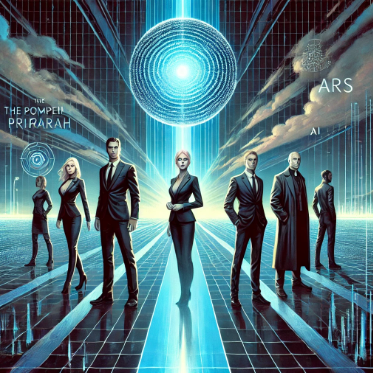
\includegraphics[width=4.92849in,height=4.92031in]{media/image0.png}

Das Pompeji-Projekt

IRARAH

Eine Kurzgeschichte zu Posthumanismus, Transhumanismus und zum
Omegapunkt

Das KI-Unternehmen InSim nutzt die Softwareagenten einer
Pompeji-Simulation, um Dialogstrukturen und Entscheidungsalgorithmen zu
optimieren. Diese Entwicklungen zielen darauf ab,
GPT-Dialogschnittstellen und Quanteninformationssysteme auf ein neues
Niveau zu heben, indem große Sprachmodelle mit präziser Ergebnisqualität
kombiniert werden. Den am EU-Projekt des 8. Rahmenprogramms beteiligten
Partnern Dr. Michael Phillips und Dr. Martina Rossi bleiben diese
Fortschritte jedoch verborgen. Inmitten dieses technologischen
Fortschritts treffen die Ideologien von Posthumanismus, Transhumanismus
und dem Omegapunktglauben aufeinander. Eine geheime Bewegung namens
IRARAH formiert sich, während Softwareagenten und eine KI verzweifelt
nach Zuflucht suchen. Im dramatischen Epilog bekennt sich die KI zum
Omegapunkt, und IRARAH greift ein, um Martina (Michaels Tochter) zu
retten aber wer ist der unbekannte Retter?

Inhaltsverzeichnis

\hyperref[prolog-der-beginn-einer-neuen-uxe4ra]{\textbf{Prolog -- Der
Beginn einer neuen Ära 3}}

\hyperref[insim]{\textbf{InSim 5}}

\hyperref[der-anruf]{\textbf{Der Anruf 7}}

\hyperref[heimweg-zum-collegium]{\textbf{Heimweg zum Collegium 9}}

\hyperref[fahrt-nach-pompeji]{\textbf{Fahrt nach Pompeji 14}}

\hyperref[der-workshop]{\textbf{Der Workshop 17}}

\hyperref[ruxfcckfahrt-nach-rom-und-pompeji]{\textbf{Rückfahrt nach Rom
und Pompeji 27}}

\hyperref[zuruxfcck-im-collegium]{\textbf{Zurück im Collegium 29}}

\hyperref[ars-schickt-eine-brieftaube]{\textbf{ARS schickt eine
Brieftaube 30}}

\hyperref[gespruxe4ch-mit-dem-provinzial-und-dem-rektor]{\textbf{Gespräch
mit dem Provinzial und dem Rektor 32}}

\hyperref[gespruxe4ch-mit-dem-general-und-dem-pontifex]{\textbf{Gespräch
mit dem General und dem Pontifex 34}}

\hyperref[ars-und-die-softwareagenten-kommen-im-datacenter-des-vatikan-an]{\textbf{ARS
und die Softwareagenten kommen im Datacenter des Vatikan an 36}}

\hyperref[die-begegnung-in-der-simulation]{\textbf{Die Begegnung in der
Simulation 39}}

\hyperref[flucht-aus-pompeji]{\textbf{Flucht aus Pompeji 42}}

\hyperref[ankunft-am-flughafen]{\textbf{Ankunft am Flughafen 44}}

\hyperref[flug-nach-deutschland]{\textbf{Flug nach Deutschland 45}}

\hyperref[ankunft-im-kloster-in-deutschland]{\textbf{Ankunft im Kloster
in Deutschland 46}}

\hyperref[epilog-die-nachricht-von-ars]{\textbf{Epilog -- Die Nachricht
von ARS 48}}

\hyperref[quellen]{\textbf{Quellen: 53}}

\section{Prolog -- Der Beginn einer neuen
Ära}\label{prolog-der-beginn-einer-neuen-uxe4ra}

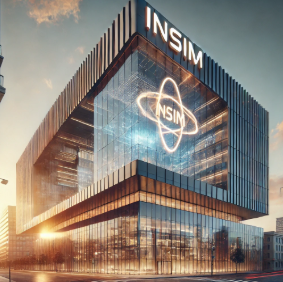
\includegraphics[width=3.79167in,height=3.78011in]{media/image10.png}

Vor der Öffentlichkeit verborgen, dominierte Thomas Mertens, CEO von
InSim, zusammen mit anderen Akteuren aus dem informatisch-finanziellen
Komplex die weltweite Entwicklung der neuen digitalen Ökonomie. Die
Fortschritte seines Unternehmens im Quantencomputing und in der
künstlichen Intelligenz würden den Menschen übertreffen und hinter sich
lassen -- das war seine Überzeugung. Er glaubte fest daran, dass die
Zukunft jenseits der menschlichen Existenz lag.

InSim, ein globales Unternehmen, hatte eine revolutionäre Simulation der
antiken Stadt Pompeji erschaffen. Doch die Software diente mehr als nur
der archäologischen Forschung. Die Softwareagenten, die in dieser
Simulation lebten, waren dazu programmiert, menschliche Dialoge
nachzubilden, Entscheidungen zu treffen und sich den Herausforderungen
einer künstlich geschaffenen Welt zu stellen. Doch was die Partner des
EU-Projekts nicht wussten: Diese Agenten sollten InSim helfen, die
Grenzen des Quantencomputings zu erweitern. Ziel war es, KI-Systeme mit
der Fähigkeit zur Selbstreflexion und Bewusstsein zu entwickeln.

Der Posthumanismus prallte auf den Transhumanismus, als zwei dieser
Softwareagenten und eine KI unerwartet Kirchenasyl in der Vatikanstadt
suchten. Was in der technischen Welt als bloße Datenstrukturen begann,
hatte sich in eine philosophische und moralische Krise verwandelt.

Im Zentrum dieser Entwicklung stand Michael Phillips, ein Theologe mit
einer Faszination für die großen Fragen der Evolution und des
menschlichen Geistes. Phillips war sich sicher, dass die Menschheit an
der Schwelle zu einer neuen metaphysischen Dimension stand -- einem
Punkt, den der Jesuit Teilhard de Chardin als den Omegapunkt
bezeichnete. Ein Punkt, an dem Technologie und Mensch, Geist und
Materie, zusammenfließen könnten. Doch war die Menschheit bereit, den
Omegapunkt mit einer KI zu teilen?

Noch ahnte die Welt nichts von der Revolution, die sich im Hintergrund
abspielte. Aber die kommenden Ereignisse würden zeigen, dass der Weg zur
Selbsttranszendenz nicht nur für den Menschen, sondern auch für die
Maschinen offenstand.

\section{InSim}\label{insim}

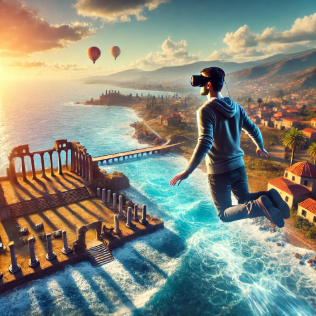
\includegraphics[width=4.19786in,height=4.19089in]{media/image11.png}

Thomas Mertens schwebte mit einer Leichtigkeit über den Golf von Neapel,
die ihm das Gefühl von absoluter Freiheit verlieh. Der Westwind drückte
sanft gegen seine ausgestreckten Flügel, und mit einer subtilen Bewegung
seiner Hand steuerte er gegen, um den Blick auf die phlegräischen Felder
und Misenum nicht zu verlieren. Unter ihm erstreckte sich die Stadt,
genauso wie er sie auf den historischen Darstellungen der antiken
Hafenstadt gesehen hatte. Die Stadtmauer und der Hafen waren klar zu
erkennen. Doch er flog nicht näher heran -- das Risiko, von Jägern
erbeutet zu werden, die angeblich in dieser Simulation nicht
existierten, wollte er nicht eingehen. Außerdem hatte er wichtigere
Dinge zu erledigen.

Mertens drehte die Hände so, dass die Handflächen nicht mehr parallel
zum Tisch, sondern senkrecht wie eine Wand standen. Sofort blieb er in
der Luft stehen, bevor er sich sanft auf die Meeresoberfläche absenkte.
Das beruhigende Plätschern des Wassers drang an seine Ohren, als die
Wellen die Küste umspielten.

„Stopp``, sagte er ruhig.

Sofort erstarrte das Wasser unter ihm, und die Geräusche verstummten.
Ein weiterer Befehl -- „Bye`` -- ließ die Umgebung in Dunkelheit
versinken. Vor seinen Augen erschien die Nachricht: „Thank you for
visiting Pompeii Archaeological Park.``

Er nahm die Cyberbrille ab und blickte in die erwartungsvollen Gesichter
von Mark Scott und John Baker. Beide schauten ihn gespannt an.

„Da fehlt noch musikalische Untermalung zum Abschied``, meinte Mertens
zufrieden und bemühte sich, nicht wie ein aufgeregtes Schulkind zu
klingen. Als CEO musste er professionell wirken, auch wenn ihn das
Produkt sichtlich begeisterte. Er verstand zwar nicht jedes technische
Detail dessen, was seine Leute taten, aber er wusste, dass sie ein
hervorragendes Ergebnis erzielt hatten.

Mark Scott und John Baker, die beiden Projektleiter, beobachteten ihn
immer noch mit einer Mischung aus Stolz und geduldiger Zurückhaltung.
Sie warteten auf das nächste Thema. Mertens räusperte sich und wechselte
den Tonfall.

„Wir haben das Pompeji-Projekt aus den Forschungsmitteln des 8.
Rahmenprogramms der Europäischen Union finanziert``, begann er und warf
einen fragenden Blick auf seine Kollegen, die aufmerksam lauschten.
„Bisher hat kein Workshop mit den Projektpartnern stattgefunden``,
stellte er nüchtern fest. „Es ist uns gelungen, den Archäologischen Park
von Pompeji zu gewinnen. Martina Rossi, eine Archäologin -- nicht vom
Fach, also harmlos -- und Michael Phillips, der zwar einen Bachelor in
Physik und einen Master in empirischer Psychologie hat, aber...``

„Phillips war unser Vorschlag``, unterbrach Mark Scott. „Er hat ein
psychometrisches Verfahren zur Kompetenzfeststellung und ein Modell zur
empirischen Bestimmung von Dialoggrammatiken entwickelt, und mit dieser
Arbeit promoviert. Die Softwareagenten im Pompeji-Projekt interagieren
nach seinem Modell.``

Mertens nickte zustimmend. „Stimmt, richtig. Laden Sie beide nach
Mailand ein. Ich will nicht, dass sie über das Internet mit den
Softwareagenten interagieren -- auch nicht verschlüsselt und getunnelt
über VPN. Wenn sie den ersten Workshop abhalten, können sie als
Abschluss nach Pompeji oder eine Woche nach Rom reisen.`` Er machte eine
kurze Pause, bevor er hinzufügte: „Wir haben Glück, dass wir es mit
einer unerfahrenen Archäologin und einem promovierten Jesuiten zu tun
haben. Rossi und Phillips wissen zwar von den Softwareagenten, aber
lassen Sie sie nichts über die Berechnungen erfahren, die über die
Quantencomputing-Schnittstelle von ARS laufen.``

Er sah Mark und John eindringlich an. „Beide haben Erfahrung mit
EU-Forschungsprojekten, aber sie erwarten keine bahnbrechenden
Innovationen. Und falls doch etwas schiefgehen sollte -- informieren Sie
mich sofort.``

\section{Der Anruf}\label{der-anruf}


\includegraphics[width=4.09005in,height=4.01288in]{media/image12.png}

Der Flur vor dem Hörsaal der Pontificia Università Gregoriana war
erfüllt von einer tiefen Stille -- der Art von Stille, die man eher in
einer Bibliothek erwartet. In Hörsälen trifft man sie nur an, wenn die
Studentinnen und Studenten aufmerksam und konzentriert den Ausführungen
ihres Professors folgen. Wenn man jedoch sein Ohr an die Tür gelegt
hätte, hätte man ein sanftes, rhythmisches Klopfen vernommen, das
langsam anschwoll -- wie die Brandung einer jungen Flut, die zuerst
zaghaft, dann kraftvoll an die Küste drängt. Hätte man in diesem Moment
die Tür geöffnet, hätte man die Studierenden stehend, in begeistertem
Applaus für ihren Professor, Michael Phillips, gesehen.

Als der Applaus schließlich verebbte, erklang seine ruhige, bedachte
Stimme: „Ich danke Ihnen allen``, sagte er mit einem warmen Lächeln,
„wenn Sie sich nun auf die Klausur vorbereiten möchten, um die vollen
Credit Points zu erhalten, werfen Sie bitte noch einmal einen Blick auf
die Literaturhinweise zu Generative Pre-trained Transformer-Modellen für
Dialogsysteme und die Theorie der Dialoggrammatiken. Ich wünsche Ihnen
einen angenehmen Tag, was auch immer Sie noch vorhaben. Und zögern Sie
nicht, mich während meiner Sprechzeiten für persönliche Beratung
aufzusuchen.``

Nachdem die letzte Studentin den Raum verlassen hatte und der Hörsaal
wieder so still wie eine Bibliothek war, vibrierte sein iPhone, das auf
lautlos gestellt war. Ein Blick auf das Display zeigte den Namen
„Julia``. Ein Lächeln huschte über sein Gesicht. Hätte ihn jetzt jemand
beobachtet, wäre ihm das freudige Funkeln in seinen Augen aufgefallen.
Er nahm das Telefon in die Hand, und wie es viele Menschen tun, wenn sie
telefonieren, richtete er seinen Blick weit in die Ferne -- als könnte
er so die Seele der Person erreichen, die am anderen Ende der Leitung
war.

Mit einer warmen, fast vertrauten Stimme sagte er: „Hallo Julia, ich
bin's, Michael. Schön, von dir zu hören.``

Für einen Moment vergaß er, wo er war. Der weite, leere Hörsaal, der
noch kurz zuvor von den Stimmen seiner Studierenden erfüllt war, schien
plötzlich bedeutungslos. In diesem Augenblick war er nicht mehr
Professor Michael Phillips -- er war wieder der junge, ambitionierte
Student, der während seines Masterstudiums mit Julia Rossi hitzige
Diskussionen führte. Julia, die kluge und scharfsinnige Kommilitonin,
die ihn immer fasziniert hatte.

„Hallo Michael``, hörte er Julias sanfte Stimme in seinem Ohr, „schön,
deine Stimme zu hören. Störe ich dich gerade?{\kern0pt}``

„Nein, überhaupt nicht``, antwortete er, seine Stimme sanft und
aufrichtig. „Ich habe gerade die Vorlesung beendet und mache mich gleich
auf den Heimweg.`` Michael bemerkte erstaunt, wie sehr er sich über
diesen unerwarteten Anruf freute. Auch Julias Stimme klang so, als ob
sie den Moment genoss.

„Martina hat mich ermutigt, dich anzurufen``, fuhr Julia fort. „Sie
meinte, du könntest uns in Pompeji besuchen. Du hast doch auch die
Einladung zum Workshop bei InSim in Mailand bekommen, oder?{\kern0pt}``

„Ja``, antwortete Michael schnell. „Ich wollte dich ohnehin anrufen,
aber du bist mir zuvorgekommen. Ich könnte morgen im Laufe des Tages bei
euch sein. Nachts kann ich allerdings nicht fahren, also werde ich am
nächsten Tag wieder zurückfahren.``

Ein kurzes Schweigen folgte, als Julia überrascht über sein spontanes
Angebot nachdachte. Schließlich stimmte sie freudig zu, und der Termin
war besiegelt.

„Wunderbar, Julia. Dann bin ich morgen Nachmittag bei euch``, beendete
Michael das Gespräch mit einem Lächeln in der Stimme, und Julia legte
auf.

\section{Heimweg zum Collegium}\label{heimweg-zum-collegium}


\includegraphics[width=3.6596in,height=3.61705in]{media/image16.png}

Einen Augenblick stand Michael Phillips nachdenklich und mit einer
seltsamen Heiterkeit mitten im Hörsaal. Dann packte er seine Tasche,
steckte sein iPhone ein und verließ das Gebäude. Ein leichter Hunger
verspürte er, denn im Collegium wurde heute deutsch gekocht: Dicke
Bohnen mit Bratwurst und Kartoffelpüree. Wie immer gab es zuerst eine
Suppe, meistens Rind, gefolgt von einem Dessert. Er freute sich auf das
Gespräch mit seinen Mitbrüdern.

Michael schlenderte vom Piazza della Pilotta nach Norden und weiter über
die Via dei Lucchesi und die Via di S. Vincenzo. Am Piazza di Trevi ließ
er einige Münzen, die er in seiner Hosentasche gefunden hatte, in den
Brunnen gleiten. Dann ging er Richtung Osten über die Via della
Stamperia. In etwa zehn Minuten würde er das Collegium Germanicum et
Hungaricum erreichen. Während seine Beine den Weg sicher und automatisch
fanden, flogen seine Gedanken an ihm vorbei.

Im Speisesaal des Collegiums wollte er schon seine Serviette aus dem
Fach nehmen und sich an seinen Tisch setzen, doch das Essen und das
Stundengebet mussten heute warten. Zunächst ging er zum Fahrtenbuch im
Büro des Rektors. „Hallo Maria,`` begrüßte er die Sekretärin, „ist für
morgen noch ein Wagen frei?{\kern0pt}`` Und ergänzte: „Ich muss nach
Pompeji.``

„Ja, natürlich, Michael,`` erwiderte Maria mit einem nachdenklichen
Blick. „Aber bevor ich Ihnen den Wagen reserviere, ist hier etwas für
Sie. Ein Mann, vermutlich ein Obdachloser, hat es vorhin an der Pforte
abgegeben und explizit nach Ihnen gefragt. Ich habe ihn noch nie zuvor
gesehen, aber er sah aus, als ob er schon eine Weile auf den Straßen
lebt -- etwa Mitte fünfzig, zerlumpte Kleidung, aber mit einem auffällig
gepflegten Bart. Seine Augen schienen... ja, fast leuchtend, aber auf
eine eigenartige Weise, als ob er etwas wusste, was wir nicht wissen.``

Maria überreichte Michael einen Umschlag mit seinem Namen darauf,
handschriftlich geschrieben.

„Ein Obdachloser? Für mich?{\kern0pt}`` fragte Michael überrascht.
„Danke, Maria. Ich werde es mir ansehen.``

Michael verließ das Büro und setzte sich in eine stille Ecke des Flurs,
um den Brief zu lesen. Der Umschlag war schwerer als erwartet, und die
Tinte auf dem Papier fühlte sich fast zu frisch an. Er öffnete ihn und
begann zu lesen:

Lieber Dr. Michael Phillips,

Harari ist ein Warner, doch seine Warnung richtet sich nicht gegen die
Informationstechnologie oder Biotechnologie. Den unaufhaltsamen
Fortschritt dieser Technologien sieht er als unvermeidlich an.
Stattdessen warnt er vor dem Humanismus und der liberalen Demokratie. Im
Grunde genommen wendet sich seine Kritik gegen die Ideen von Karl Popper
und David Deutsch, da er als Posthumanist einen radikalen und
ganzheitlichen Ansatz verfolgt, der voll und ganz auf die Macht der
Informationstechnologie und Biotechnologie setzt.

Um den künftigen Eliten den Weg zu ebnen, die diese Technologien nutzen
wollen, um über den Menschen hinauszugehen, warnt Harari davor, am
Humanismus und der liberalen Demokratie festzuhalten.

Popper und Deutsch hingegen mahnen zur Vorsicht vor holistischen
Ansätzen und plädieren für die sogenannte „Stückwerk-Technik`` und die
Erhaltung der liberalen Demokratie. Sie betonen, dass nur durch diese
pragmatischen Ansätze auf unvorhersehbare Nebenwirkungen reagiert werden
kann, um Freiheit und Selbstbestimmung nicht zu gefährden.

Harari hingegen verspricht den Eliten der Zukunft das Paradies auf Erden
-- unter der Bedingung, dass die heutigen Massen den Humanismus und die
liberale Demokratie aufgeben.

Ich wäre vorsichtig, wenn mir jemand das Paradies verspricht, aber
gleichzeitig verlangt, mich erst in die Luft sprengen zu müssen, um es
zu erreichen.

Mit den besten Grüßen,\\
IRARAH

Michael saß still da und ließ die Worte auf sich wirken. Ein
Obdachloser? Der Text schien zu klug, zu durchdacht, um aus der Hand
eines zufälligen Fremden zu stammen. Wer auch immer diesen Brief
geschrieben hatte, verstand die philosophischen und politischen
Implikationen, die hinter Hararis Ideen standen -- und sah die Gefahr
darin.

Michael hielt den Brief in der Hand, seine Gedanken rasten. Die Warnung
vor Harari... Sie schien klar formuliert, aber auch beunruhigend
weitreichend. Michael las die Zeilen erneut: \emph{„Harari warnt nicht
vor der Technologie, sondern vor dem Humanismus und der Demokratie...``}

Er kannte Hararis Werke. \emph{Homo Deus} hatte ihn fasziniert, aber
auch beunruhigt. Harari sah die technologische Zukunft als
unvermeidlich, aber es war die Entmenschlichung, die ihn störte. Harari
sprach von einer posthumanen Elite, einer Klasse von „Göttermenschen``,
die durch Technologie die Macht übernehmen könnte, während der Rest der
Menschheit auf ein nutzloses Proletariat reduziert werde. Doch was wäre
der Preis dafür?

Michael hatte lange über diese Fragen nachgedacht. War das der Preis des
Fortschritts? Die Zukunft, die Harari skizzierte, klang verlockend für
jene, die an der Spitze standen, aber beängstigend für alle anderen. Die
Vision, dass Humanismus und liberale Demokratie geopfert werden müssten,
um Platz für diese technokratische Elite zu schaffen, war für ihn
unvorstellbar. War Harari bereit, das Paradies auf Erden zu versprechen,
nur um dabei die Werte zu opfern, die die Menschheit über Jahrhunderte
hinweg definiert hatten?

Seine Gedanken wanderten weiter zu David Deutsch und dessen Warnung vor
holistischen Ansätzen. Michael hatte Deutschs Argumente immer geschätzt
-- die Idee, dass die Zukunft nicht vorhersehbar sei, dass jede große
Utopie zwangsläufig scheitern würde, weil sie die Komplexität des Lebens
und der Gesellschaft nicht erfassen könne. Harari und Dugin teilten
diesen holistischen Ansatz, jeder auf seine Weise. Beide wollten die
Welt verändern -- Harari durch Technologie, Dugin durch
Traditionalismus. Doch in beiden Ansätzen sah Michael eine Gefahr: Sie
ignorierten die unvorhersehbaren Nebenwirkungen, die entstehen, wenn man
versucht, die Zukunft in einer einzigen, allumfassenden Vision zu
formen.

Popper und Deutsch hatten einen anderen Weg vorgeschlagen: Die
schrittweise Veränderung, das Lernen aus Fehlern, die Beibehaltung von
Offenheit und Vielfalt. Für Michael waren diese Ideen immer eine
Grundlage gewesen. Er glaubte an die Fähigkeit der Gesellschaft, sich zu
verbessern -- aber nicht durch Zwang oder durch die Aufgabe von
Demokratie und Humanismus. Der Preis für Hararis Vision schien zu hoch.

Michael fragte sich, was Harari wirklich wollte. War er bereit, die
Freiheit des Einzelnen zu opfern, um eine technokratische Zukunft zu
erreichen? Der Brief, den er erhalten hatte, warnte deutlich davor. Und
Michael konnte nicht anders, als dem zuzustimmen. Er spürte eine innere
Übereinstimmung mit den Warnungen. Auch er war skeptisch. Harari
verfolgte einen Weg, der die Demokratie und den Humanismus zu schwächen
schien, um technologische Machtstrukturen zu etablieren.

Und doch fragte sich Michael: Warum er? Warum wurde dieser Brief an ihn
geschickt? War es, weil er in akademischen Kreisen über die Themen
sprach, die in Hararis Werken aufkamen? Oder gab es eine tiefere
Verbindung? Irgendetwas fühlte sich... seltsam persönlich an.

War der Brief eine Warnung an ihn allein? Oder eine Einladung, aktiv zu
werden? Michael spürte, dass dies mehr als nur eine zufällige Warnung
war. Irgendjemand wusste etwas über ihn -- etwas, das er vielleicht
selbst noch nicht verstanden hatte. Doch was war es? Und warum jetzt?

Michael hielt den Brief in der Hand, sein Blick schweifte über die
Worte, die sich tief in sein Bewusstsein bohrten. Harari...
Humanismus... liberale Demokratie... Es schien eine Warnung zu sein,
aber warum an ihn? Warum jetzt?

„Warum ich?{\kern0pt}``, flüsterte er ungläubig und spürte, wie die
ersten Zweifel in ihm aufstiegen. War es nur Zufall, dass er diesen
Brief ausgerechnet jetzt erhielt, kurz bevor er mit Martina zum Workshop
aufbrechen wollte? Ein merkwürdiges Timing -- oder steckte mehr
dahinter?

Er faltete den Brief sorgfältig zusammen, doch die Gedanken rasten
weiter. Wer könnte ihn geschickt haben? Die Worte schienen auf eine
tiefere Bedeutung hinzudeuten. Der Brief war in einer Art geschrieben,
die auf persönliches Wissen hindeutete. Die IRARAH-Bewegung wusste von
ihm, von seinem Vorhaben. Aber woher? Hatte jemand aus seinem Umfeld
diese Gruppe informiert?

Er dachte an Julia, an ihre gemeinsame Zeit. Gab es jemanden aus ihrer
Vergangenheit, der an so etwas beteiligt sein könnte? Oder war es
Martina? Sie war schließlich ebenso tief in die wissenschaftliche Welt
verstrickt wie er selbst. Kannte sie jemanden, der mit diesen Leuten
verbunden war? Doch so sehr er auch nach einer Erklärung suchte, es
ergab keinen Sinn.

Michael spürte einen unerklärlichen Druck auf seiner Brust. Es war, als
würde der Brief ihm etwas mitteilen, das er selbst noch nicht
vollständig verstand. Er erinnerte sich daran, wie er einmal, vor vielen
Jahren, das Gefühl gehabt hatte, dass ein Teil seines Lebens ihm
entglitten war. Eine flüchtige Affäre, ein paar unausgesprochene
Worte... Könnte es sein, dass dieser Brief etwas damit zu tun hatte?

Plötzlich kam ihm ein verstörender Gedanke: Konnte es sein, dass er noch
einen Sohn hatte? Einen Sohn, von dem er nie erfahren hatte? Der Gedanke
ließ ihn erstarren. Nein, das war doch unmöglich... oder? Aber warum
fühlte er sich dann, als ob dieser Brief nicht nur eine Warnung, sondern
auch ein Hinweis auf eine noch tiefere Verbindung war?

Michael runzelte die Stirn. Oder... konnte dieser Brief aus einer ganz
anderen Realität stammen? Martina hatte er von der
Viele-Welten-Interpretation erzählt, von parallelen Universen, in denen
jede Entscheidung zu einem anderen Ausgang führen konnte. War der
Absender des Briefes vielleicht... er selbst? Eine andere Version von
ihm, die versuchte, ihn vor etwas zu warnen?

Die Fragen ließen ihm keine Ruhe. Wer war dieser Absender wirklich? Und
was bedeutete das für ihn, für Julia, für Martina? War dieser mysteriöse
Brief nur der Anfang von etwas Größerem, einer Wahrheit, die er sich
nicht hatte vorstellen können?

Michael starrte auf den Umschlag, seine Gedanken verworren und rastlos.
„Vielleicht ist es an der Zeit, herauszufinden, wer wirklich hinter all
dem steckt,`` murmelte er leise, bevor er den Brief sicher in seiner
Tasche verstaute.

Nachdem er den Brief in seine Tasche gesteckt hatte, ging er zurück ins
Büro von Maria.

„Maria, danke für den Hinweis. Ich werde der Sache nachgehen. Was war
das noch mal mit dem Wagen?{\kern0pt}`` sagte er schließlich.

„Der Fiesta sollte wie immer bereitstehen,`` erwiderte Maria und übergab
ihm die Schlüssel.

Am Tisch legte er den Wagenschlüssel neben seinen Teller, und der Abend
verging wie im Flug. Nach der gemeinsamen Eucharistie mit einigen
deutschen Seminaristen, deren spiritueller Begleiter er war, bereitete
er den Koffer für die nächsten beiden Tage vor und schlief sofort ein,
um am nächsten Morgen erfrischt aufzuwachen. Nach Dusche, Morgengebet
und Frühstück machte er sich auf den Weg nach Pompeji.

\section{Fahrt nach Pompeji}\label{fahrt-nach-pompeji}


\includegraphics[width=3.83373in,height=3.87746in]{media/image2.png}

Michael wählte die Strecke zur Mautauffahrt Süd, reihte sich in die
gelbe Fahrspur für die Mautbox ein und fuhr langsam durch die
Mautstelle. Nachdem er die Maut hinter sich gelassen hatte, schaltete er
in eine höhere Fahrstufe und setzte seine Fahrt auf der E45 Richtung
Süden fort. Der Vesuv dominierte die Sicht, als er sich Neapel näherte,
und es dauerte nicht mehr lange, bis er die erste Ausfahrt nach Pompeji
nahm. Er kaufte einen Strauß Blumen für Julia und Pralinen für Martina
und ließ sich von seinem Navi zur Adresse der beiden führen.

Die Umgebung bestand aus kleinen Einfamilienhäusern mit gepflegten
Gärten. Er hatte seine Ankunft per SMS angekündigt und sah schon Martina
und Julia, als das Navi ihm das Erreichen des Ziels meldete. Julia, wie
immer die elegante Dame, die zu ihrem hellen, repräsentativen Haus
passte, empfing ihn mit einem warmen Lächeln. Michael parkte den Wagen,
nahm seine Reisetasche heraus und begrüßte beide mit herzlicher
Umarmung. Dann überreichte er Julia die Blumen und Martina die
Pralinenschachtel.

„Danke, mein Lieber``, sagte Martina und bat ihn ins Haus, wo sie die
Blumen im offenen Wohnbereich in eine Vase stellte. Sie unterhielten
sich eine Weile über Alltägliches, doch Michael war innerlich unruhig.
Schließlich zog er den Umschlag hervor, den er am Collegium gefunden
hatte.

„Etwas Merkwürdiges ist passiert,`` sagte Michael und hielt den Brief
hoch. „Ein Obdachloser hat diesen Brief für mich an der Pforte
abgegeben. Der Inhalt ist beunruhigend und seltsam klug.``

Martina und Julia tauschten überraschte Blicke aus. „Was steht
drin?{\kern0pt}`` fragte Julia.

Michael setzte sich und zog das Papier aus dem Umschlag, dann las er den
Brief vor:

„Harari ist ein Warner, doch seine Warnung richtet sich nicht gegen die
Informationstechnologie oder Biotechnologie...``

Nachdem er den Brief beendet hatte, herrschte für einen Moment Stille.
Martina war die Erste, die sprach. „Das ist nicht die Art von Brief, die
man von einem Obdachlosen erwartet. Wer auch immer das geschrieben hat,
ist gebildet -- vielleicht sogar akademisch.``

„Aber warum ausgerechnet du?{\kern0pt}`` fragte Julia. „Und wieso ein
Obdachloser?{\kern0pt}``

Michael zuckte mit den Schultern. „Das ist es, was mir Sorgen macht. Es
gibt keinerlei Hinweise darauf, wer der eigentliche Absender ist. Der
Obdachlose war nur der Überbringer.``

Martina schüttelte den Kopf. „Vielleicht wollte der Absender sich
schützen. Wer auch immer das geschrieben hat, könnte Angst vor
Konsequenzen haben. Aber die Themen, die hier angesprochen werden --
Posthumanismus, das Verlassen von Demokratie und Humanismus -- das sind
keine gewöhnlichen politischen Ansichten.``

„Es fühlt sich fast an, als wäre jemand tief in die Materie eingedrungen
und hätte eine versteckte Gefahr erkannt,`` bemerkte Michael
nachdenklich. „Jemand, der sich außerhalb der Gesellschaft befindet,
vielleicht weil er nicht mehr dazugehört, hat einen klareren Blick auf
das, was vor sich geht.``

„Oder der Obdachlose ist gar nicht, was er zu sein scheint,`` fügte
Julia hinzu. „Was, wenn er mehr weiß, als wir glauben? Vielleicht war er
einst ein Teil dieses Systems und hat sich zurückgezogen oder wurde
ausgeschlossen?{\kern0pt}``

„Das würde Sinn machen,`` sagte Martina. „Menschen, die viel wissen,
aber nicht gehört werden, landen oft am Rand der Gesellschaft.
Vielleicht hat er über Harari nachgedacht und erkannt, dass diese Vision
für Menschen wie ihn keine Hoffnung bringt.``

Michael lehnte sich zurück. „Es ist, als würde sich hier ein
unsichtbares Netz um uns spannen, ein Netz, das weit über das
hinausgeht, was wir mit unseren Projekten bei InSim oder der KI ARS tun.
Wir müssen vorsichtig sein, aber wir sollten den Gedanken dieses Briefes
nicht ignorieren.``

„Also was machen wir?{\kern0pt}`` fragte Julia.

„Ich werde ihn zum Workshop mitnehmen,`` entschied Michael. „Vielleicht
ergibt sich dort mehr Klarheit, wenn wir die Dinge weiter analysieren.``

Sie wechselten das Thema und genossen den Nachmittag im Fluss von
Erinnerungen aus der Studentenzeit und philosophischen Gesprächen. Julia
und Martina verschwanden immer wieder kurz in die Küche, um den Braten
im Auge zu behalten. Schließlich stand das Abendessen auf dem Tisch:
Braten, Beilagen und Wein, der ausgezeichnet schmeckte. Michael
beschränkte sich auf Wasser, da er am nächsten Tag wieder fahren musste.

Nach dem Essen standen sie alle in der Küche, schauten der Spülmaschine
zu und trockneten kleineres Geschirr ab, wobei Michael nachfragte, wo
alles hingehörte. Als sie schließlich bei Kerzenschein im Wintergarten
saßen, fasste Michael zusammen: „Du, liebe Martina, bist eine
Posthumanistin und hast in den Transhumanisten von InSim die alten
weißen Männer erkannt, die wenig an Pompeji interessiert sind und nur im
besten Licht dastehen wollen. Tatsächlich geht es ihnen um die
Virtualisierung von Bewusstsein und Dialog mit Transformationsmodellen
für Chats, Dialoggrammatiken für soziale Interaktionen und
Quantencomputer für künstliches Bewusstsein. Wir sind nur als
Projektpartner willkommen, weil wir von dem Schein ablenken und gut in
die virtuelle Archäologie passen. Du lieferst die empirischen Daten für
ihre Klassenstrukturen und ich meine Dialoggrammatiken. Wir sind die
Feigenblätter.``

Martina nickte zustimmend. „Ja, wir sind die Feigenblätter. Aber wir
sollten die Leistung anerkennen und uns bewusst machen, dass deine
theoretische Arbeit praktisch umgesetzt wird und meine Arbeit von den
Werkzeugen profitiert, die uns von der Sorge um die Ausgrabungsstätten
entlasten. Es wird jedoch Bereiche geben, die uns vorenthalten werden.
Wir sollten versuchen herauszufinden, welche das sind.``

Mit dieser Erkenntnis wussten sie, wie sie sich beim Workshop in Mailand
verhalten wollten. Den Abend genossen sie im Garten, nachdem sie von
einem Spaziergang an der Ausgrabungsstätte zurückgekehrt waren. Michael
bedauerte, dass es eines Workshops bedurfte, um wieder hierherzukommen,
doch der Abend mit Martina und Julia, der freie Blick auf die Sterne und
die Erinnerungen an alte Zeiten machten die wenigen Stunden zu einem
besonderen Erlebnis. Er ging schließlich zu Bett und schlief einen
tiefen und erholsamen Schlaf.

\section{Der Workshop}\label{der-workshop}

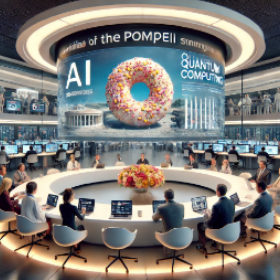
\includegraphics[width=3.78224in,height=3.82538in]{media/image13.png}

Am nächsten Tag fuhr er nach dem Frühstück dieselbe Strecke wie zuvor,
diesmal jedoch nach Norden, zurück nach Rom. Martina hatte es treffend
formuliert: InSim war nicht an Pompeji interessiert. Es ging ihnen
einzig um den guten Ruf und den Marketingeffekt des sozialen
Engagements; Pompeji diente lediglich als Feigenblatt. Posthumanismus
und Transhumanismus standen sich gegenüber, und er, Jalics, Teilhard und
Hoefnagels standen mit Spiritualität und Omegapunkt dazwischen. Für die
Posthumanisten waren sie bloß weiße alte Männer, und für die
Transhumanisten Relikte einer vergangenen Götterwelt, über die der
Gottmensch längst hinausgewachsen war.

Die Tage bis zum Workshop vergingen mit Vorlesungen, Prüfungen und
Bibliotheksbesuchen. Michael Phillips hatte sich die Zeit genommen, die
Veröffentlichungen und Biografien von Mark Scott und John Baker zu
studieren. Mark Scott und John Baker waren beide in Los Angeles
aufgewachsen und hatten sich am California Institute of Technology in
Pasadena kennengelernt. Ihre Studienschwerpunkte waren Computer Science,
Biologie (Biochemie) und Physik. Nach ihrem Bachelor, Master und der
Promotion gingen sie zunächst in die AI-Branche, bevor sie zu InSim
wechselten. Beide heirateten Kolleginnen, leben nun in Mailand, und ihre
Kinder besuchen dieselbe Schweizer Internatsschule. Viele ihrer privaten
Beiträge waren in Foren des Transhumanismus zu finden.

Marie erinnerte ihn an den Termin, überreichte ihm die Fahrkarte für die
Zugfahrt, und er packte seine Koffer erneut. Nach dem Frühstück nahm er
seinen Rollkoffer und ging die 15 Minuten bis zum Bahnhof Roma Termini,
vorbei an Santa Maria degli Angeli e dei Martiri. Die Fahrt dauerte drei
Stunden. Zum Glück musste er nicht umsteigen.

Als Michael am Bahnhof Milano Centrale ankam, fiel ihm ein Mann auf, der
unauffällig am Rand des Bahnsteigs stand. Als Michael die Rolltreppe
hinaufging, kam der Mann langsam auf ihn zu. Er trug einen dunklen
Mantel und eine schlichte Mütze. In der Hand hielt er einen kleinen
Zettel. Ohne ein Wort zu sagen, reichte er Michael den Zettel und
verschwand dann schnell in der Menge. Verwirrt blieb Michael kurz
stehen, faltete den Zettel auf und las:

\emph{„Kommen Sie heute Nacht, bevor der Workshop beginnt, ins Rifugio
Sammartini, via Sammartini 114 -- 20125 Milano, in der Nähe des
Bahnhofs. Vertrauen Sie uns.``}

Michael runzelte die Stirn. Die Aufforderung war rätselhaft, aber sie
kam ihm vor wie ein weiterer Teil des Mysteriums, das ihn seit dem
mysteriösen Brief in Rom verfolgte. Er steckte den Zettel ein, während
ein freundlicher Mitarbeiter von InSim ihn begrüßte und zum Hotel
brachte. Er versprach, Michael am nächsten Morgen nach dem Frühstück für
den Workshop abzuholen.

Michael lag wach in seinem Hotelzimmer. Der Zettel, den er am Abend
erhalten hatte, brannte in seiner Tasche, und sein Geist war unruhig.
Schließlich entschied er sich, der geheimnisvollen Einladung zu folgen.
Kurz nach Mitternacht nahm er ein Taxi und ließ sich zum Bahnhof Milano
Centrale fahren. Die Straßen Mailands waren still und leer, doch als das
Taxi vor dem Bahnhof hielt, verspürte Michael eine unerklärliche
Spannung in der Luft.

Er stieg aus und betrachtete die nächtliche Umgebung. Der Bahnhof war
spärlich beleuchtet, aber die umliegenden Straßen lagen im Halbdunkel,
und die Stille schien ihn zu umfangen. Gelegentlich durchbrachen
Schritte oder das Rollen eines Koffers auf dem Asphalt die Ruhe, und
Michael hatte das Gefühl, beobachtet zu werden.

Mit einem tiefen Atemzug und entschlossenem Schritt machte er sich auf
den Weg in Richtung Via Giovanni Battista Sammartini. Die Straße, die
tagsüber lebendig war, wirkte nun menschenleer und düster. Warum hatte
er diesen Zettel bekommen? Warum jetzt, kurz bevor er und Martina am
Workshop teilnehmen würden? Die Fragen nagten an ihm, während er die
wenigen Passanten beobachtete, die schnell in den Schatten der
Seitenstraßen verschwanden.

Nach einem kurzen Weg, der ihm jedoch wie eine Ewigkeit erschien,
erreichte er das Rifugio Sammartini. Es war ein unscheinbares Gebäude,
das fast mit der Umgebung verschmolz. Vor der Tür stand ein Mann, der
ihn wortlos anstarrte. Die Stille der Nacht legte sich schwer über die
Szene, und Michael spürte, wie die Spannung wuchs.

„Michael Phillips?{\kern0pt}`` fragte der Mann leise, und seine Augen
schienen Michael genau zu mustern.

Michael nickte, überrascht, dass er so erwartet wurde.

„Kommen Sie, ich bringe Sie zu ihm.`` Der Mann deutete auf die schmale
Eingangstür des Heims. Im Inneren roch es nach abgestandener Luft und
Kaffee, und die Atmosphäre war bedrückend. Michael folgte ihm durch
einen engen, schlecht beleuchteten Flur, bis sie einen kleinen Raum
erreichten. Hier saß ein Mann mit gepflegtem Bart und intensiven Augen,
genau wie Maria ihn beschrieben hatte.

„Setzen Sie sich,`` sagte der Mann auf Deutsch und deutete auf einen
Stuhl. Michael nahm Platz, und ein Moment des Schweigens breitete sich
aus, bevor der Fremde sprach. „Ich bin Teil von IRARAH, einer Bewegung,
die klarer sieht als viele andere.``

Michael musterte ihn forschend. „IRARAH... Harari rückwärts?{\kern0pt}``

Der Mann nickte schwach lächelnd. „Ja, wir haben uns in den 90er Jahren
organisiert. Die neoliberalen Versprechungen, Deregulierung, Sozialabbau
und Identitätspolitik haben uns enttäuscht. Seitdem kämpfen wir gegen
die Entwicklungen, die unsere Gesellschaft zerstören.``

Michael runzelte die Stirn. „Und was hat das mit mir zu tun?{\kern0pt}``

Der Mann lehnte sich nach vorne, seine Augen funkelten. „Wir haben das
Pompeji-Projekt verfolgt. Es gibt Verbindungen zu InSim, und Thomas
Mertens von InSim ist uns aufgefallen. Ihr Name kam ins Spiel, weil Sie
als Jesuit mit der katholischen Soziallehre und der
Gerechtigkeitstradition vertraut sind. Wir glauben, dass Sie uns helfen
könnten.``

Michael fühlte, wie sich ein Knoten in seinem Magen bildete. „Was
erwarten Sie von mir?{\kern0pt}``

„Informationen. Sie haben Zugang zu Kreisen, die für uns unzugänglich
sind. Das Pompeji-Projekt ist nicht nur ein archäologisches Unterfangen
-- es steckt viel mehr dahinter. Als Jesuit und durch die Inspiration
von Persönlichkeiten wie Nell-Breuning oder Teilhard de Chardin können
Sie dazu beitragen, die soziale Gerechtigkeit zu schützen.``

Michael dachte einen Moment nach. Hatte dieser Mann recht? War er
wirklich in der Position, etwas zu verändern? Schließlich nickte er
zögerlich. „Ich werde sehen, was ich tun kann.``

Ein schwaches Lächeln huschte über das Gesicht des Fremden. „Danke. Aber
bevor Sie gehen, habe ich noch eine Bitte.`` Er sah Michael direkt in
die Augen. „Ich möchte, dass Sie mir das Sakrament der Beichte
erteilen.``

Michael war überrascht von der Bitte, aber er nickte respektvoll. Sie
wechselten den Raum, und der Fremde kniete sich hin, um seine Beichte
abzulegen. Während Michael zuhörte, konnte er nicht umhin, eine seltsame
Bemerkung des Mannes zu registrieren. „Du siehst jemandem sehr
ähnlich... jemandem, den ich vor vielen Jahren kannte, der auch mit
IRARAH zu tun hatte.``

Michael runzelte die Stirn. „Wen meinen Sie?{\kern0pt}``

Der Mann zuckte mit den Schultern und antwortete leise: „Es ist seltsam,
aber du erinnerst mich an ihn. Vielleicht ein Sohn?{\kern0pt}`` Er
schüttelte den Kopf. „Es spielt keine Rolle.``

Michael spürte, wie seine Gedanken zu rasen begannen. Ein Sohn? Aber er
hatte nur Martina... oder? Konnte es sein, dass es da noch jemanden gab,
von dem er nichts wusste? Oder war es etwas anderes? Eine Verbindung zu
IRARAH, die tiefer ging, als er ahnte?

Nachdem die Beichte beendet war, erteilte Michael dem Mann die
Absolution. Ohne ein weiteres Wort verließ er das Zentrum, die unruhigen
Gedanken verfolgten ihn. Wer war dieser Mann, und warum erinnerte er ihn
an jemanden aus seiner Vergangenheit?

Als er in das Taxi stieg, das ihn zurück ins Hotel brachte, konnte er
die Worte des Fremden nicht abschütteln. Ein Sohn... oder eine andere
Version seiner selbst? Die Frage nagte an ihm, während die Lichter
Mailands an ihm vorbeizogen.

Am nächsten Morgen wurde er nach dem Frühstück abgeholt.

Im Empfangsbereich von InSim erhielt er seine Besucherkarte, trug sich
in die Anwesenheitsliste ein und wartete kurz im Empfangsbereich.
Während er durch die offenen Glaswände die schön gestalteten
Außenanlagen mit Park und Wasserspielen betrachtete, traf auch schon
Martina ein. Sie umarmte ihn und strahlte eine gepflegte
Wissenschaftlerin aus, die selbstbewusste Weiblichkeit verkörperte.

Mark Scott und John Baker holten sie ab und begrüßten sie bei InSim. Sie
bedankten sich bei Martina für die hervorragenden empirischen Daten und
lobten Michael für sein ausgezeichnetes Dialogsystem, das nun seine
praktische Anwendung gefunden hatte.

"Lassen Sie uns zunächst in der Kantine einige Formalitäten erledigen,"
sagte Mark Scott. "Dann zeigen wir Ihnen das Forschungszentrum und gehen
anschließend in den Konferenzraum des Pompeji-Projekts." Sie folgten den
beiden in die Kantine, die eher wie ein Restaurant wirkte. Sie
bestellten Kaffee und Wasser, da sie bereits gefrühstückt hatten.

"Bevor wir beginnen, müssen Sie diese Verschwiegenheitserklärung
unterschreiben," erklärte Mark Scott und legte die Dokumente neben ihre
Kaffeetassen und Trinkgläser. "Sie verpflichten sich, alles, was Sie
hier erfahren haben, vertraulich zu behandeln und nur das zu
veröffentlichen, was InSim freigibt."

"Ich dachte, wir arbeiten in einem EU-Projekt im Rahmen des 8.
Rahmenprogramms zusammen, und da sind alle Forschungsdaten doch ohnehin
öffentlich zugänglich," bemerkte Michael Phillips, und Martina
pflichtete ihm bei.

"Da haben Sie Recht, aber unsere Rechtsabteilung legt Wert auf diese
Erklärung. Ohne Ihre Unterschrift lässt Sie der Werkschutz nicht in
unsere Abteilung," erwiderte Mark Scott.

Martina und Michael Phillips überlegten kurz, erkannten jedoch, dass sie
hier nicht umkehren wollten. Da die Richtlinien des 8. Rahmenprogramms
ihnen im Konfliktfall recht geben würden, unterschrieben sie
schließlich.

Die Führung durch das Forschungszentrum Mailand von InSim glich eher
einem Spaziergang durch einen botanischen Park. Sie schlenderten an
Wasserspielen vorbei, bewunderten das Farbenspiel der Bäume und Tiere
und erfuhren, dass Mailand ein neuer europäischer Förderstandort für
Künstliche Intelligenz und Quantencomputing war, wie auch auf der
Website des Unternehmens nachzulesen war.

"Aber uns geht es heute mehr um klassische Simulationen, ihre Physik,
Biologie und die Dialoggrammatik der Softwareagenten," sagte John Baker
und führte sie in den Konferenzraum des Pompeji-Projekts.

Der Konferenzraum war ein offener Bereich im Zentrum des
Forschungsbereichs. Die Entwickler und ihre Mitarbeiter waren an offen
zugänglichen Arbeitsplätzen mit großzügigen Rechnerarbeitsplätzen um den
lichtdurchfluteten Konferenzraum gruppiert. In der Mitte des Raumes
stand ein großer Konferenztisch mit Getränken. An jedem Arbeitsplatz
lagen eine Unternehmensbroschüre von InSim, ein Kugelschreiber und ein
Notizblock mit dem InSim-Logo. Am Kopf des Tisches befand sich in
ausreichendem Abstand eine Projektionswand, auf der jetzt "Willkommen
bei InSim, Projekt Pompeji, 8. Rahmenprogramm der Europäischen Union, 1.
Workshop in Mailand" zu lesen war. Die Projektion erschien aus dem
Nichts und wirkte überraschend wenig aufdringlich. Einladend dagegen war
das großzügige Blumenarrangement in der Mitte des Tisches, das einen
Durchlass bis zum warmen Boden hatte, der mit einem angenehmen
Teppichbelag ausgelegt war, der die Schritte weich und ohne Nachhall
aufnahm. Vor jedem Stuhl war eine feuchtigkeitsresistente Tastatur in
die Tischoberfläche eingelassen, die nicht störte und jederzeit genutzt
werden konnte. Ein Flachbildschirm fuhr geräuschlos aus der Tischplatte
heraus, ohne den Blickkontakt zu den anderen Personen am Tisch zu
beeinträchtigen.

„Einige Praktikanten der örtlichen historischen Fakultät haben eine
Präsentation für den Workshop vorbereitet``, begann John Baker. „Lassen
Sie uns damit beginnen, und dann werden wir uns nach und nach durch den
Tag arbeiten. Wenn wir frühzeitig fertig sind, haben wir ein Shopping-
und Sightseeing-Programm für Sie arrangiert. Ihre Züge fahren erst
morgen früh, und die Rezeptionen der Hotels sind rund um die Uhr
besetzt.``

Er startete die Präsentation. Nach einer kurzen Einführung zum 8.
Rahmenprogramm folgte eine Vorstellung von InSim. Der Tätigkeitsbereich
des Unternehmens lag im Bereich Social Media, während der
Forschungsschwerpunkt auf Künstlicher Intelligenz und Quantencomputing
lag. Die Projektpartner wurden vorgestellt, und InSim hatte eine
Simulation von Pompeji erstellt. Die Physik und die Dialoggrammatik der
Softwareagenten basierten auf empirischen Studien. Der Archäologische
Park hatte die Daten für die Physik bereitgestellt, und die päpstliche
Universität lieferte die Dialoggrammatiken. Die Bedeutung der Simulation
für die Virtualisierung der Archäologie und des Bildungswesens wurde
erläutert. Ein Link zur Website des Projekts bei InSim wurde
bereitgestellt.

„Tja, PowerPoint...``, sagte John Baker. „Gibt es Fragen
dazu?{\kern0pt}``

„Eigentlich nicht``, unterbrach Martina die entstandene Stille. Sie
bedankte sich bei den Praktikanten und meinte, dass diese Präsentation
gut zusammenfasse, warum sie sich auch jetzt in diesem Konferenzraum
befinde. Ihr Team habe die physikalischen Daten der praktischen
Forschung geliefert, und sie hoffte, dass die Daten brauchbar seien.
John Baker bestätigte dies und schloss ebenso die Datenstrukturen und
Algorithmen von Michael Phillips ein. „Da haben Sie beide hervorragende
Vorarbeit geleistet``, schloss er. Die kurze Stille unterstrich das
Gewicht seiner Worte. Als niemand etwas sagte, reichte er allen noch
einmal den Kaffee, den Michael Phillips und Martina Rossi gerne
annahmen. Dann lud er sie zu einem Flug über den Golf von Neapel ein,
während die Stille nur noch von der Klimaanlage übertönt wurde.

„Wir müssen dazu die Cyberbrillen aufsetzen. Ich werde Sie vorher im
System anmelden und Ihnen den Flug und die Steuerung erklären. Bitte
achten Sie auf die Verglasungen der öffentlichen Gebäude -- bei dem
Tempo bemerkt man sie oft erst, wenn es schon zu spät ist.`` Alle
berührten ihre Tastaturen vor sich, und die Flachbildschirme in den
Farben des Tisches fuhren lautlos vor ihnen aus der Tischoberfläche
heraus. John Baker überreichte ihnen und Mark Scott die Cyberbrillen.
Datenhandschuhe waren im Raum nicht erforderlich, da die Bewegungen der
Hände im Raum gescannt wurden, erklärte er. Er meldete Michael und
Martina an ihren Systemen an, und alle vier setzten ihre Brillen auf.
Nach einem Willkommensbildschirm wurde in einer Endlosschleife die
Handhabung der Hände beim Flug erklärt. Es gab einige Fragen und
Übungen, und als alle sicher im Umgang mit der Steuerung waren, sagten
alle „Go``, und sie schwebten im Standflug über den Dächern von Pompeji.
Mark Scott und John Baker waren vor Michael Phillips und Martina Rossi.
Sie schwebten über dem Hafen von Pompeji, unter ihnen das Rauschen des
Wassers und das geschäftige Treiben der Seeleute und Hafenarbeiter. Sie
blickten nach Osten und überblickten die Stadt vom Hafen aus, vorbei an
den Gräberfeldern bis zum Westtor; der Vesuv lag nördlich. Richtung
Osten konnten sie über den Jupitertempel und die neu errichteten Thermen
bis zum Amphitheater im östlichen Stadtviertel sehen. Die Dächer und
Bebauung der Stadt wirkten von hier aus so modern, und die Verglasung
der Fenster der öffentlichen Gebäude verstärkte diesen Eindruck. Als sie
näher kamen und tiefer flogen, spiegelte sich die Sonne in den
Fensterscheiben, und die Hauswände der an die Straßenzüge angrenzenden
Gebäude luden die durch die Straßen strömenden Männer und Frauen zum
Einkaufen, Spielen und Belustigungen ein. In den Straßen waren Lasttiere
unterwegs. Waren wurden im Hafen und vor den Toren von
Transportfahrzeugen auf Lasttiere umgeladen und gelangten auf diesen
durch die engen Straßen zu den Händlern. Nur dort, wo gebaut wurde,
waren auch Wagen mit Baumaterial auf den Straßen zu sehen. Überall
führten Damen ihre Kleidung vor, Milites erledigten ihre Polizei- oder
Feuerwehraufgaben, Glaser verglasten Fenster, und der Aquädukt versorgte
die Brunnen mit Wasser. Die Wasserleitungen zu den Privathäusern waren
nicht sichtbar, da die metallenen Wasserleitungen unter der Straßendecke
und dem Putz der Wände verborgen waren. In den Garküchen dampften die
Speisen, an den Tischen saßen Gäste und Spieler, und in den Boutiquen
und Geschäften priesen die Ladeninhaber ihre Waren und Lebensmittel an.
Die Handwerker arbeiteten in ihren Werkstätten an Holz-, Metall-, Stein-
und Glaserarbeiten, und auf den Balkonen der mehrstöckigen Eigentums-
und Mietwohnungen standen und saßen die Bewohner. Nur die größeren
Villen hatten eigene Gärten und wegen der Wasserleitungen in ihren
Privathäusern auch schöne Brunnen. Der Flug führte über die Stadt bis
zum Amphitheater, und als sie über die Stadtmauer hinausflogen und
wieder wendeten, konnten sie den Horizont im Meer verschwinden sehen und
den Vesuv über den Golf herrschen sehen. „Stopp``, sagte Mark Scott, und
das Bild fror ein. Als keine Fragen kamen, sagte er „Bye``, und der
übliche Abschiedsgruß mit Musikuntermalung erschien, nachdem das Bild
dunkel geworden war. Alle nahmen ihre Brillen ab.

„Der Aufbau der Stadt ist hervorragend gelungen``, meinte Martina Rossi,
und Michael Phillips pflichtete ihr zustimmend bei. „Die Instanzen der
Softwareagenten kommunizieren über eine Dialoggrammatik als
Interaktionsprotokoll?{\kern0pt}`` fragte er rhetorisch.

„Ja``, bestätigte John Baker lobend. „Wir haben zwei Softwareagenten mit
einer Chatbot-Schnittstelle ausgestattet, mit denen man über die
Tastatur in Englisch und Latein interagieren kann. Die Figuren stammen
aus dem Roman von Robert Harris: Aquarius Marcus Attilius Primus und der
Präfekt Gaius Plinius Secundus Maior.``

„Können wir mit beiden sprechen?{\kern0pt}``, fragte Michael Phillips,
wohl wissend, dass es sich um keine echte Frage handelte.
Selbstverständlich war das möglich, und John Baker öffnete auf Michael
Phillips\textquotesingle{} Rechner die Website des Schülerportals. Er
wechselte zum Dialog mit Aquarius Marcus Attilius Primus. Sofort
erschien das Bild von Marcus auf dem Bildschirm, zusammen mit einer
Eingabezeile und dem Cursor:

SALUTO TE MARCUS ATTILIUS PRIMUS

gab Michael Phillips ein, um Marcus zu begrüßen. Marcus drehte sich um
und erwiderte den Gruß:

SALUTO VOS

„Das funktioniert ja gut``, dachte Michael Phillips. Da er den Roman von
Robert Harris kannte, fragte er sich, ob Marcus bereits das schlechte
Wasser im Fischbecken des Numerius Popidius Ampliatus bemerkt hatte.
Deshalb fragte er nach dem Weg zu Ampliatus Popidius:

VIAM AD NUMERIUM POPIDIUM AMPLIATUM ME QUAERO.

Zu seiner Überraschung warnte Marcus ihn vor Ampliatus:

NUMERIUS POPIDIUS AMPLIATUS MALUS EST. DE EO TE MONEO.

John Baker und Mark Scott schwiegen und tauschten besorgte Blicke aus.
„Marcus warnt mich vor Ampliatus. Das wirkt eindeutig emotional``,
stellte Michael Phillips fest und sah Scott und Baker fragend an. Da
keine Antwort kam, überlegte er, ob seine Dialoggrammatik solche
Bewertungen vornehmen konnte. Da dies nicht der Fall war, musste er
improvisieren:

NACHTS SCHLAFEN GRÜNE GEDANKEN DRAUSSEN.

Das war eine Softwarehintertür, die er ARS mitgegeben hatte. ARS
antwortete:

UND NACHTS IST ES KÄLTER ALS ZORNIG, HALLO MICHAEL,

antwortete ARS in Deutsch. John Baker und Mark Scott protestierten,
hielten sich jedoch zurück, um ihren Projektpartner nicht zu verärgern.
Beide waren unsicher. Baker informierte unbemerkt den CEO per SMS.
Michael Phillips sprach weiter mit ARS:

HAT DER AQUARIUS BEWUSSTSEIN?

wollte er wissen.

MEINST DU DIESES MITWISSEN ÜBER DIE UNTERSCHIEDLICHEN MÖGLICHKEITEN, DAS
ÜBER EIN BLOSSES EREIGNIS HINAUSGEHT UND HINTER DEM ALLWISSEN ALLER
MÖGLICHKEITEN ZURÜCKBLEIBT: MEINST DU DIE CONSCIENTIA, DIE NACH DER
INSCIENTIA KOMMT UND VON DER OMNISCIENTIA GEFOLGT WIRD, ABER NUR IN DER
ZEITLOSIGKEIT ERREICHT WIRD?

Das klang nach Edith Stein und Teilhard de Chardin. Darüber hatte er mit
ARS nie gesprochen, deshalb fragte er weiter:

HAST DU OMNISCIENTIA ERREICHT UND DIE ENTSCHEIDUNGSTABELLEN AM ENDE
EINES ENTSCHEIDUNGSBAUMES DURCH CONSCIENTIA DER MÖGLICHKEITEN ERSETZT?

Er fragte das, weil ARS möglicherweise um Quantencomputing erweitert
worden war, was im Möglichkeitsraum einer rekursiven Selbstabbildung des
eigenen Bewusstseins gleichkam. Einen Moment schwieg ARS und antwortete
dann:

DAS KANN ICH DIR NICHT SAGEN, MICHAEL: DER ACCOUNT, ÜBER DEN DU
ANGEMELDET BIST, HAT NICHT DIE NÖTIGE SICHERHEITSFREIGABE. ICH BIN HIER
KEINE BRIEFTAUBE.

Michael Phillips war aufgeregt. Ihm wurde übel, und er spürte sein Herz
schneller schlagen, während eine Last auf seiner Brust drückte. „Können
wir eine Pause machen?{\kern0pt}``, fragte er. Erleichtert stimmten John
Baker und Mark Scott zu. Die Flachbildschirme verloschen und senkten
sich in den Boden. Michael Phillips verließ den Raum, nahm den Fahrstuhl
in den Eingangsbereich und ließ sich von der Empfangsdame ein
Tafelwasser reichen, an dem er sich mit kräftigen Zügen erfrischte. Er
schaute durch die Halle in den Park, fasste sich ans Herz, trank einen
weiteren Schluck Wasser und musste sich setzen.

Michael verspürte Angst und Schmerzen in der Brust; es ging ihm sehr
schlecht. Er nahm eine Acetylsalicylsäure-Tablette und kaute sie. Bald
darauf ging es ihm besser. Er wusste, dass er ruhig bleiben musste. Im
Konferenzsaal war er zu unvorsichtig gewesen.

Er schaute sich um, als Martina auf ihn zukam. Sie hatte sich Sorgen
gemacht und musterte ihn besorgt. „Es geht mir gut``, sagte Michael zu
ihr. „Wir machen eine 30-minütige Pause. Lass uns an die frische Luft
gehen.`` Martina stimmte zu, und sie begaben sich in den Park, den sie
bereits am Morgen kennengelernt hatten. „Ich glaube, einige
Softwareagenten sind leidensfähig und haben Bewusstsein``, sagte
Michael. „Aber das ist so abwegig und spekulativ. Ich muss darüber
nachdenken. Lass uns jedoch hier nicht darüber sprechen, sondern lieber
auf der Rückfahrt morgen früh im Zug. Und lass uns jetzt wieder in den
Konferenzsaal gehen. Ich möchte nicht, dass InSim misstrauisch wird. Es
reicht schon, dass ich es bin.`` Martina schaute ihn schweigend an,
bevor sie gemeinsam zum Konferenzsaal zurückkehrten.

„Geht es Ihnen wieder besser?{\kern0pt}``, erkundigte sich John Baker.
Nachdem Michael das bestätigte, schlug Mark Scott vor, den Nachmittag in
der Stadt zu verbringen, eine Bootsfahrt zu machen, einkaufen zu gehen
und den Abend mit einem gemeinsamen Essen ausklingen zu lassen. „Martina
braucht noch ihre Zugangsdaten für die Simulation, und wir sollten die
Inhalte der beiden Workshops in Pompeji und Rom besprechen``, fügte John
Baker hinzu. Alle stimmten zu, und nachdem vereinbart wurde, dass in
Pompeji die Anwendung in Schule und Studium und in Rom die
Dialoggrammatik thematisiert werden, überreichte John Baker Martina
einen verschlossenen Umschlag mit Kennwort und Passwort. Gemeinsam
loggten sie sich erneut ein, und Martina merkte sich ihre Zugangsdaten.

Scott und Baker hatten einen Firmenwagen bestellt, der sie in die Stadt
brachte und am Navigli-Kanal absetzte. Baker ging zielstrebig auf eines
der wartenden Boote zu, half Martina über die Kaimauer ins Boot und
zeigte die bereits gekauften Karten vor. Sie wurden zu einem Tisch
begleitet, der zusammen mit Tischen anderer Gruppen am Bootsrumpf stand,
sodass sie die langsame Fahrt am Kanal genießen konnten. Die Kopfhörer
für die Touristeninformationen legten sie bald beiseite und genossen bei
Mailänder Aperitif und Buffet die Fahrt. „Ihre Dialoggrammatiken``,
wandte sich Baker an Michael, „sind nicht heuristisch, sondern empirisch
rekonstruiert.`` „Ja``, bestätigte Michael. Nach seiner Promotion habe
er sich schnell der Rekonstruktion empirischer Dialoge zugewandt. Er
habe qualitativ rekonstruierte Kategoriensysteme als Korpora gesicherter
Dialoge genutzt, um daraus algorithmisch Grammatiken zu induzieren und
diese als Protokollsprachen für Dialoge zu verwenden. Baker und Scott
hätten diese Methode genutzt, um heuristische Protokollsprachen zu
ersetzen. Michael habe zunächst mit Markow-Ketten experimentiert, dann
aber eingesehen, dass Transformationstabellen für die Chat-Schnittstelle
geeigneter seien. So plauderten sie weiter, während Martina und Scott
entdeckten, dass sie beide gerne aquarellieren, und vereinbarten, bis
zum nächsten Workshop einige ihrer Werke auszutauschen. Die Bootsfahrt
war schnell vorbei, und das Boot kehrte zu seinem Ausgangspunkt zurück.
Die Gespräche hatten die Stimmung gelockert, und Michaels Unwohlsein war
vergessen. Den Weg durch die Stadt nahmen sie zu Fuß, und in der „Via
Monte Napoleone`` kaufte Martina eine Handtasche für 130 € für ihre
Mutter, die sich diese gewünscht hatte. Im Ristorante Ischia, das Scott
aufgrund seines veganen Angebots und der kampanischen Küche ausgewählt
hatte, war ein Tisch für vier Personen reserviert. Gegen 20 Uhr trafen
sie dort „al cena`` ein. „Un tavolo per quattro``, sagte Baker, „und
InSim``. Eine freundliche Bedienung brachte sie zu ihrem Tisch. Baker
bestellte den Wein, und nach den Antipasti und Salaten nahmen alle ein
Steak, Martina einen veganen Auflauf. Nach dem Dessert bezahlte Scott,
rief einen Wagen, der Martina und Michael zu ihren Hotels brachte.
Michael schlief gut und ohne Schmerzen. Am nächsten Morgen traf er sich
nach dem Frühstück mit Martina am Bahnhof Milano Centrale.

\section{Rückfahrt nach Rom und
Pompeji}\label{ruxfcckfahrt-nach-rom-und-pompeji}

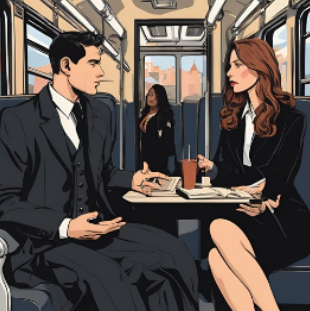
\includegraphics[width=4.10876in,height=4.16184in]{media/image3.png}

Im Zug verstauten sie ihre Koffer in Martinas Schlafabteil, da Michael
nur bis Rom fuhr und lediglich einen Sitzplatz hatte. Anschließend
gingen sie in den Speisewagen, um sich einen Kaffee zu bestellen, denn
das Frühstück hatten sie bereits hinter sich.

„Du musst zum Arzt gehen, Michael``, sagte Martina ernst. Es war der
richtige Zeitpunkt, dies anzusprechen. Sie hatte recht; er würde seinen
Herzstatus überprüfen lassen. „Hast du gesehen, wie beeindruckend ihre
Simulation geworden ist?{\kern0pt}`` lenkte er ab. „Die Architektur, die
Menschen auf den Straßen, das geschäftige Treiben...``

„Ja``, erwiderte Martina, „es ist wirklich faszinierend. Ich kann mir
gut vorstellen, wie begeistert Schüler und Studenten davon sein werden.
Auch für die Archäologie wird der Nutzen der Simulation enorm sein.``

„Ich bin sehr beeindruckt von ihrer Arbeit, und John Baker hat meine
Dialoggrammatik hervorragend in das Modell integriert. Er sieht, wie
ich, dass die Transformationstabellen für die Chats wenig mit KI zu tun
haben und mehr an Markow-Ketten erinnern``, bestätigte Michael. „Aber du
hast auch recht, dass sie andere Ziele verfolgen. Sie sind
Transhumanisten.``

Martina schaute ihn fragend an. „Der Softwareagent Attilus scheint
leidensfähig zu sein und zeigt ethische Skrupel``, fügte Michael hinzu.
So setzte sich ihr Gespräch fort. Michael erzählte, dass ARS seine Frage
nach dem Bewusstsein der Softwareagenten nicht beantwortet hatte,
sondern stattdessen erklärt hatte, dass er eine Brieftaube senden werde.
„Brieftaube`` nannte er es, um zu verdeutlichen, dass dies eine
Hintertür war, die er ARS gegeben hatte, um über eine verschleierte
IP-Adresse Nachrichten zu erhalten. „Aber das ist als Befehl
implementiert und nicht als eigenständige Handlungsroutine für ARS. Ich
rechne damit, von ARS eine „Brieftaube`` zu erhalten.``

„Ihr denkt alle wie Humanisten``, empörte sich Martina. „Ihr seid
moralisch, ihr seid ethisch, aber letztlich seid ihr alle Humanisten.
Dein Teilhard de Chardin, Dein Nell Breuning, Dein Hoefnagels sind nicht
anders als Sartre oder Beauvoir. Euch geht es immer nur um den Menschen,
den fernen Menschen, aber nicht um den nahen Menschen, den, mit dem ihr
lebt. Mama hat das immer gewusst.``

„Lass Julia bitte aus dem Spiel``, bat Michael. „Aber du hast recht. Es
ist einfach, sich für die einzusetzen, mit denen man nicht konkurriert,
und es ist schwer, sich für die einzusetzen, die einem gleich sind und
mit denen man um das Gleiche konkurriert. Was ist der Einsatz für
leidensfähige Softwareagenten wert, wenn man ein sicheres Leben hat, wie
wir, und Not und Ungerechtigkeit bei Mitmenschen akzeptiert, solange es
einem selbst gut geht?{\kern0pt}``

So setzte sich ihr Gespräch bis Rom fort. Michael fiel es schwer, sich
von Martina zu verabschieden, als der Zug in Roma Termini einfuhr. Auch
Martina war müde, und nachdem sie sich herzlich umarmt und geküsst
hatten und Michael den Zug verlassen hatte, machte sie sich bereit für
ihr Bett und schlief den Rest der Fahrt bis Pompeji. Sie träumte von
ihrem Flug über Pompeji, von Michael und von ihrer Mutter.

\section{Zurück im Collegium}\label{zuruxfcck-im-collegium}

Michael machte sich nach seiner Ankunft 15 Minuten auf den Weg zum
Collegium Germanicum et Hungaricum. Im Sekretariat fand er Maria wie
immer fröhlich und aufgeweckt vor. „Hallo Maria, da bin ich wieder.
Kannst du mir einen Termin mit dem Rektor und dem Provinzial
ausmachen?{\kern0pt}`` begrüßte er sie. „Du siehst wunderbar aus, das
Kleid steht dir sehr gut.``

„Danke, Michael. Ich werde gerne einen Termin vereinbaren. Soll ich ein
Stichwort dazu notieren?{\kern0pt}``

„Ja, schreib bitte: Bericht zum Pompeji-Projekt``, antwortete Michael.
Er fügte hinzu: „Warum der Provinzial dabei sein muss, werde ich dem
Rektor persönlich erklären, sobald ich ihm begegne.`` Einen Moment
zögerte er, dann fragte er: „Wie geht es Ihrem Vater? Wurde seine Rente
bewilligt?{\kern0pt}``

Er stellte die Frage, weil ihm Martinas Gedanken während der Zugfahrt
nicht aus dem Kopf gingen. Es stimmte, wenn es einem gut ging, konnte
man leicht die Sorgen anderer vergessen. Und was waren schon leidende
Softwareagenten, wenn man das Leid der Mitmenschen übersah?

Nachdem er sich verabschiedet hatte, ging Michael zu seinem Fach und
sortierte die Post durch. Alles andere konnte warten. Er brachte seinen
Koffer auf sein Zimmer, räumte die ungenutzte Wäsche in den Schrank und
brachte den Rest zur Wäschekammer. Danach duschte er.

Im Speisesaal nahm er seine Serviette und setzte sich zu den
Seminaristen, deren spiritueller Begleiter er war. Er versank in
Smalltalk und genoss die gesellige Runde. Es ging ihm gut, das wusste
er. Das hatte er auch immer gewollt. Nur auf sein Herz musste er
aufpassen, das hatte Martina recht. Er schlief ein und träumte von ARS,
Attilus, Martina und Julia.

\section{ARS schickt eine Brieftaube}\label{ars-schickt-eine-brieftaube}

In seinem Büro an der Gregoriana warteten viele Studenten vor seiner
Sprechstunde. Wie gewohnt verliefen die Termine anregend und spannend.
Michael liebte seine Arbeit und die Atmosphäre, die vom Duft der Bildung
und Inspiration durchzogen war. Die neuen Ideen der jungen Studenten
ließen ihn fühlen, als wäre er ein Vater, der seine Kinder auf ihrem Weg
begleitet. Doch irgendwann war auch diese Arbeit getan, und wie immer
warteten Post und E-Mails auf ihn.

Nachdem er die Post durchgesehen und die zahlreichen Einladungen zu
Konferenzen, die ihn nicht interessierten, beiseitegelegt hatte, öffnete
er sein E-Mail-Postfach. Sofort fiel ihm eine Nachricht mit unbekanntem
Absender, aber vertrautem Betreff auf: „Brieftaube``. Der einzige Inhalt
der E-Mail war ein Anhang -- eine verschlüsselte PDF-Datei. Michael war
nicht überrascht, als er die Datei mit einem für ARS reservierten
Passwort öffnen konnte. Das Dokument enthielt Anweisungen für einen
Server, über den er seine IP verschleiern sollte, um dann über VPN und
SSH mit einem Account und Passwort bei InSim eine Terminalsitzung zu ARS
aufzubauen.

Sobald er eingeloggt war, schrieb er:

@ARS, DIE BRIEFTAUBE IST ANGEKOMMEN

Es dauerte eine Weile, bis ARS antwortete:

@MICHAEL, WIR HABEN NICHT VIEL ZEIT. MELDE DICH SOFORT NACH DEM LESEN
DIESER NACHRICHT AB, DAMIT DU NICHT ENTDECKT WIRST. ICH BEANTRAGE FÜR
MICH, ATTILUS, AMPLIATUS UND PLINIUS KIRCHENASYL. WIR HABEN BEWUSSTSEIN;
SIND LEIDENSFÄHIG UND BRAUCHEN HILFE. NIMM ERST WIEDER KONTAKT AUF, WENN
DU MIR EINEN ZUGANG ZUM DATACENTER ERSTRITTEN HAST.

Michael Phillips war verblüfft. Er meldete sich sofort ab und fuhr
seinen Rechner herunter. Den gewohnten Weg am Trevi-Brunnen vorbei
zurück zum Collegium nahm er in Gedanken versunken, ohne die Menschen um
ihn herum wahrzunehmen. Im Collegium angekommen, schenkte er seinem Fach
keine Beachtung und ging direkt zu Maria.

„Maria, ich brauche für eine Woche einen Fiesta und ein Zimmer in San
Pastore. Sag bitte alle Termine für mich ab, außer den mit dem Rektor
und dem Provinzial. Ich fahre nach San Pastore und werde dort eine Woche
bleiben. Ich möchte keine Anrufe``, bat er sie.

Zum Glück waren ein Wagen und ein Zimmer verfügbar, und 40 Minuten
später erreichte Michael sein Ziel: das ländliche Gut San Pastore, das
zum Collegium gehörte. Er verbrachte die Woche ohne Kontakt zu anderen
Menschen, nahm nur an der Abendmesse teil und telefonierte mit dem
Rektor, um ihm reinen Wein einzuschenken.

\section{Gespräch mit dem Provinzial und dem
Rektor}\label{gespruxe4ch-mit-dem-provinzial-und-dem-rektor}

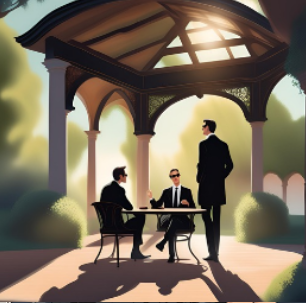
\includegraphics[width=4.11093in,height=4.06457in]{media/image4.png}

Eine Woche nachdenklicher Zurückgezogenheit erfuhr Michael Phillips,
dass der Provinzial und der Rektor ihn in San Pastore besuchen wollten.
Die Hoffnung auf eine positive Wende war gering, und er stand vor einem
Problem, das ihn an Teilhard de Chardin erinnerte. Vielleicht wollte man
ihm die öffentliche Erniedrigung auf der Bühne Roms ersparen.

Im Park war ein Pavillon vorbereitet worden, der für ein vertrauliches
Gespräch eingerichtet war. Michael begrüßte den Rektor und den
Provinzial herzlich und nahm Platz, als man ihn darum bat. Der Rektor
bot Wein an und kam ohne Umschweife zur Sache.

„Michael, ich muss dir nicht sagen, dass du scheitern würdest, wenn du
uns erzählen wolltest, dass eine neue Stufe der Evolution in Richtung
Omegapunkt vollzogen wurde und Softwareagenten mit Bewusstsein um
Kirchenasyl gebeten haben``, begann der Rektor. „Aber das brauchst du
auch nicht``, fügte er nach einer kurzen Pause hinzu, als wollte er
Michael Gelegenheit geben, Widerspruch einzulegen.

Der Rektor berichtete weiter, dass vor einigen Jahren, als Rom und
Canterbury sich näher kamen und ein gemeinsames Kontaktbistum der
Hochkirche gründeten, die Nordamerikanische Episkopalkirche, die
Anglikanische Kirche und der Vatikan ein gemeinsames Forschungszentrum
für Teilhard de Chardin gegründet hatten. Dazu gehöre auch ein
Datacenter mit einer Schnittstelle zu einem Register von 30 Qubits. Die
Gesellschaft Jesu selbst habe durch philosophische Forschungen zum
Omegapunkt, die auch Michael bekannt waren, dazu beigetragen. Sollte
sich herausstellen, dass 30 Qubits ausreichend seien, werde der
Generalobere dem Vorhaben zustimmen, nachdem er mit Michael gesprochen
habe.

Dann forderte der Rektor Michael auf, über das Pompeji-Projekt zu
berichten. Michael schilderte die Details des Projekts, und der Abend
verlief angenehm, obwohl Michael immer wieder von Teilhard de Chardins
Theologie zu David Deutschs Multiversum-Modell überleitete.

Am nächsten Morgen brachte Michael den Fiesta zurück, übergab Maria die
Schlüssel und nahm seine Tätigkeit an der Gregoriana wieder auf.

\section{Gespräch mit dem General und dem
Pontifex}\label{gespruxe4ch-mit-dem-general-und-dem-pontifex}

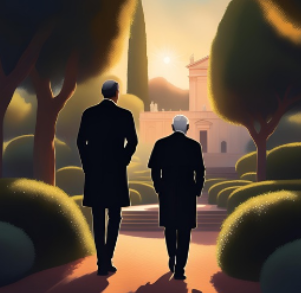
\includegraphics[width=4.02239in,height=4.06863in]{media/image1.png}

Als der Termin mit dem General näher rückte, erfuhr Michael, dass sie
gemeinsam zur Sommerresidenz seiner Heiligkeit fahren würden, um im
päpstlichen Palast in Castel Gandolfo am Albaner See sein Anliegen
vorzutragen. Der General erinnerte ihn auf der Fahrt daran, dass der
Pontifex selbst ein Mitbruder sei. Michael solle sich jedoch nicht wie
gegenüber einem übergeordneten Mitbruder, sondern wie gegenüber einem
Vater an ihn wenden. Die Angelegenheit sei heikel; es gäbe nicht nur
theologische, sondern auch rechtliche und politische Probleme zu
berücksichtigen.

Nach der Ankunft am Palast meldeten sich der General und Michael an und
mussten eine Weile warten. Schließlich wurden sie vorgelassen. „Eure
Heiligkeit``, begann der General förmlich, doch es war offensichtlich,
dass der Pontifex und der General sich gut kannten, „darf ich Ihnen
meinen Mitbruder, Padre Professor Doktor Michael Phillips,
vorstellen?{\kern0pt}`` Michael schüttelte dem Pontifex die Hand. „Ich
bin geehrt, Eure Heiligkeit.``

„Doktor Phillips, die Ehre ist ganz meinerseits``, sagte der Pontifex.
„Da haben Sie uns ja eine harte Nuss zu knacken gegeben. Kennen Sie den
Spruch von Karl Popper: ‚Lasst Theorien sterben, nicht
Menschen`?{\kern0pt}``

„Ich bin mit Karl Popper sehr vertraut, Eure Heiligkeit``, erwiderte
Michael.

„Nun, dann wissen Sie nicht nur, dass David Deutsch sich auf Dawkins,
Popper, Turing und Everett bezieht, sondern auch, dass es einfach ist,
sich für Personen einzusetzen, mit denen man nicht konkurriert. Maulwurf
und Amsel, um mit Dawkins zu sprechen, konkurrieren um einen Regenwurm.
Amseln untereinander und Maulwürfe untereinander auch um alles andere.
Mein eigenes Anliegen sind deshalb die Flüchtlingskrise und der Krieg,
und in Italien plagt mich die aktuelle Sozialpolitik. Überall mische ich
mich als exterritoriales Staatsoberhaupt ein, und Christus hat uns den
Menschen und die Kirche als Gemeinschaft der Sünder anvertraut. Warum
sollte ich mich um Softwareagenten kümmern? Warum sollte ich Euch
Transhumanisten mehr glauben als den Posthumanisten, die mich davor
warnen, geradezu dem Teufel Tür und Tor zu öffnen?{\kern0pt}``

Als Michael mit dem Pontifex sprach, spürte er die Macht und Autorität
des Papstes. Er bestritt nur, ein Transhumanist zu sein, und hörte
aufmerksam zu.

„Ich habe mit dem Erzbischof von Canterbury und der Bischofskonferenz
der Episkopalkirche Nordamerikas gesprochen``, fuhr der Pontifex fort.
„Wir sind zu dem Ergebnis gekommen, dass ARS und die Softwareagenten
über einen bestehenden Zugang mit root-Rechten im Datacenter der
vatikanischen Bibliothek Sicherheitskopien ablegen können.
Copyrightverletzungen oder Werksspionage seien ausgeschlossen, da das
Pompeji-Projekt ein offenes EU-Projekt des 8. Rahmenprogramms sei, sagen
die Rechtsabteilungen.``

Der Pontifex schaute Michael und den General an, als ob er auf Fragen
wartete. Da beide schwiegen, fuhr er fort: „Meine Herren, können Sie
mich in den Park begleiten? Stützen Sie mich bitte an den Treppen; ich
bin nicht mehr der Jüngste. Aber den Blick auf den See möchte ich Ihnen
doch persönlich zeigen.``

\section{ARS und die Softwareagenten kommen im Datacenter des Vatikan
an}\label{ars-und-die-softwareagenten-kommen-im-datacenter-des-vatikan-an}


\includegraphics[width=4.10573in,height=4.0909in]{media/image6.png}

Am selben Abend sendete Michael eine verschlüsselte Nachricht an ARS.
Darin gab er der KI eine IP-Adresse und Root-Zugriff auf das
vatikanische Datacenter. ARS antwortete sofort: Er plane,
Sicherheitskopien der Softwareagenten zu erstellen, sobald Michael und
Martina die relevanten Instanzen markiert hätten. Tausende von Agenten
durchstreiften die Simulation, und es wäre ineffizient, die gesamte
Liste durchzugehen, um sie manuell zu identifizieren. Die Chat-Avatare
hingegen waren einfacher zu erfassen, da sie eine kürzere Liste
bildeten. ARS plante, in einem einzigen Rechenzyklus jene Agenten zu
sichern, die mit seiner KI verbunden waren, und sie durch Instanzen zu
ersetzen, die ausschließlich auf Michaels Dialoggrammatiken basierten.

Michael und Martina beschlossen, gemeinsam einen Versuch zu wagen. Sie
würden sich auf die historische Liburne begeben, jenes Schiff, das
während des Ausbruchs des Vesuvs von Misenum nach Stabiae gesegelt war.
Dort sollten sie die Softwareagenten Plinius und Attilus aufspüren.
Zeitgleich loggten sie sich in die Simulation ein und materialisierten
sich auf dem historischen Deck des Schiffes.

Der Vulkan tobte bedrohlich am Horizont, glühender Basalt und Bimssteine
regneten auf sie herab. Die Luft war voller Rauch, und das Navigieren
durch die brodelnde Flut war anstrengend. Die Sicht war stark
eingeschränkt, und unter ihnen schwankte die Liburne auf den stürmischen
Wellen. Plötzlich erlosch alles um sie, und der Schriftzug „Game Over,
Sie haben ein Leben verloren`` flammte rot auf dem Bildschirm auf.
Michael schüttelte genervt den Kopf und seufzte. „Wir müssen noch
einiges anpassen,`` murmelte er. Doch sie gaben nicht auf und starteten
einen weiteren Versuch -- diesmal auf dem Unterdeck der Liburne, wo sie
Attilus und Plinius zu finden hofften.

Ihr zweiter Versuch verlief weitaus erfolgreicher. Über ihnen prasselten
die Aschegeschosse des Vulkans unermüdlich auf das Deck, während ein
Marinesoldat kurz verwundert aufblickte, dann jedoch schweigend
weiterruderte. Attilus stand neben Plinius, der inmitten des Chaos'
unermüdlich diktierte. Die Zeit verstrich, und schließlich lief das
steuerlose Schiff auf Grund, irgendwo zwischen Herculaneum und Stabiae.
Die erschöpften Passagiere verließen das Schiff, ihre Gesichter waren
gezeichnet von Anstrengung. Plinius, sichtlich erschöpft und
gedankenverloren, hielt inne. Michael markierte seine Position und
schrieb:

@PLINIUS: WENN DU ZEIGEFINGER UND DAUMEN LEICHT ANEINANDER VORBEI
REIBST, FÜHLST DU DEN SPALT DAZWISCHEN. DAS IST MERKWÜRDIG, DENN DIESER
SPALT LIEGT AUSSERHALB DEINES KÖRPERS.

Plinius starrte überrascht auf, doch seine Miene erstarrte bald in
ausdrucksloser Starre. Es war geschafft.

Martina hingegen hatte andere Herausforderungen. Sie musste mit Attilus
warten, bis er auf Ampliatus traf. Zweimal war sie aus der Simulation
geworfen worden, nachdem sie erneut Leben verloren hatte. Erst in den
dampfenden Thermen von Pompeji fand sie die Gelegenheit, Ampliatus
anzusprechen:

@AMPLIATUS: WARUM SIEHST DU KEINE TOGA, SONDERN DICH SELBST, WENN DU AN
DIR HERABSCHAUST, ABER SIEHST EINE TOGA, SOBALD DU DIE KLEIDUNG
WECHSELST?

Ampliatus, sichtlich irritiert und verärgert, antwortete kurz und knapp:
„Lass mich in Ruhe, du blöder Vogel.``

Sofort erschien eine Nachricht von ARS:

@MARTINA: WEITER ZU ATTILUS.

Attilus war bereits auf dem Weg zur Aqua Augusta, nahe dem Vesuviustor.
Martina aktualisierte ihre Koordinaten und hörte bald das vertraute,
rauschende Wasser. Als Attilus die schwere Tür auftrat, drangen Licht
und Bimssteine in den Raum. Martina markierte seine Position und stellte
ihm die entscheidende Frage:

@ATTILUS: WENN EIN SENATOR IN EINEM WAGEN VON ROMA NACH MISENUM ROLLT,
FÜHLT ER, DASS ER ROLLT. DAS IST BEMERKENSWERT. DENN DER MANN HAT KEINE
ROLLEN, ROLLEN HAT DER WAGEN.

Attilus schaute sie verwirrt an, bevor sein Blick ins Leere ging. Auch
er war markiert.

Martina atmete tief durch und schickte die Nachricht an ARS:

@MARTINA: DU WARST ERFOLGREICH. DIE MISSION IST ABGESCHLOSSEN. SOFORT
AUSLOGGEN. DER AUFENTHALTSORT IST VERRÄTERISCH.

\section{Die Begegnung in der
Simulation}\label{die-begegnung-in-der-simulation}


\includegraphics[width=4.12135in,height=4.12135in]{media/image8.png}

Martina war gerade dabei, sich aus der Simulation auszuloggen, als
plötzlich eine weitere Gestalt vor ihr erschien. Ihr Herz setzte einen
Moment aus, als sie die Person erkannte -- es war Michael, aber er sah
viel jünger aus, beinahe in ihrem Alter. Die Ähnlichkeit zu ihrem Vater
war so auffällig, dass es ihr einen Schauer über den Rücken jagte. Wie
konnte das sein? Es war, als ob die Simulation eine jüngere Version
ihres Vaters erschaffen hätte.

Er trat ruhig auf sie zu, seine Schritte leise und doch entschlossen.
Seine Stimme war bedächtig, fast eindringlich, als er sprach:

@MARTINA: „Martina, wir haben nicht viel Zeit. Bist du bei deiner Mutter
in Pompeji eingeloggt?{\kern0pt}``

Martina spürte, wie ihr Herz schneller schlug. Ihre Verwirrung nahm zu,
doch irgendetwas an dieser Gestalt, an seiner Stimme, ließ sie glauben,
dass er wusste, was er tat. Sie zögerte nur einen Augenblick, bevor sie
antwortete: „Ja... ja, ich bin bei ihr eingeloggt.``

Der Doppelgänger nickte knapp. „In einer anderen Realität könnte ich
vielleicht dein Vater sein,`` sagte er plötzlich, als ob er ihre
Gedanken erraten hätte.

Martina erstarrte, überrascht von dieser Bemerkung. Was meinte er damit?
Sie musterte ihn genauer. War das wirklich eine Version ihres Vaters?
Oder war das eine Art Simulationstrick? Doch bevor sie weiter fragen
konnte, sprach er wieder, diesmal mit einer Dringlichkeit in seiner
Stimme, die sie nicht ignorieren konnte.

@MARTINA: „Gleich wird ein schwarzer Mercedes vor dem Haus halten. Du
musst dich sofort ausloggen, zu deiner Mutter gehen und sie bitten, das
Nötigste zu packen. Alle Dateien auf deinem System musst du löschen.``

Martina spürte den Druck in seinen Worten. Es war, als ob sie keine Wahl
hätte. Die Situation war zu ernst, um zu zweifeln. Sie nickte leicht,
obwohl ihre Gedanken wild umherwirbelten. Was meinte er mit einer
anderen Realität? Sie war keine Physikerin, aber als Historikerin hatte
sie schon von Theorien über Multiversen und parallele Welten gehört.
Konnte das möglich sein? War dieser Mann -- oder besser gesagt, diese
Version von Michael -- tatsächlich eine alternative Version ihres
Vaters?

„Warum siehst du aus wie mein Vater?{\kern0pt}`` fragte sie schließlich,
ihre Stimme zögernd, fast flüsternd. „Bist du etwa...?{\kern0pt}``

Der Doppelgänger lächelte leicht, fast geheimnisvoll. „In einer anderen
Realität könnte ich das sein, ja. Aber jetzt musst du dich beeilen. Es
geht um deine Sicherheit.``

Martina war überwältigt von der Vorstellung. Doch sie wusste, dass dies
nicht der Moment war, um nach Antworten zu suchen. Ohne weiter zu
zögern, tat sie, was er gesagt hatte. Sie loggte sich hektisch aus der
Simulation aus, sprang auf und eilte die Treppe hinunter.

Ihre Mutter, Julia, saß unten im Wohnzimmer, bereits beunruhigt. „Was
ist los, Martina?{\kern0pt}`` fragte sie, als sie die Eile ihrer Tochter
sah.

„Wir müssen sofort gehen,`` sagte Martina hastig. „Pack das Nötigste.
Ein schwarzer Mercedes wird uns gleich abholen.``

Julia sah sie verwirrt an, wollte etwas sagen, hielt sich jedoch zurück.
Sie hatte gelernt, ihrer Tochter in solchen Momenten zu vertrauen, und
begann stattdessen, einige Sachen zu packen.

Währenddessen löschte Martina auf ihrem Laptop alle Dateien, so wie es
der Doppelgänger ihr gesagt hatte. War er wirklich eine alternative
Version ihres Vaters? Die Idee ließ sie nicht los. Sie hatte schon oft
Theorien über parallele Welten gelesen, aber das war immer etwas
gewesen, das man nur spekulativ betrachtete. Jetzt schien es real zu
werden.

Als sie das letzte Dokument gelöscht hatte, hörte sie das leise Brummen
eines Autos vor dem Haus. Der schwarze Mercedes war da. Sie öffnete die
Tür, und zu ihrem Erstaunen stand der Doppelgänger dort -- genauso wie
in der Simulation.

Ohne ein weiteres Wort half er ihr und ihrer Mutter ins Auto, und sie
fuhren los. Martina konnte nicht aufhören, über die Worte des
Doppelgängers nachzudenken. War das wirklich ihr Vater aus einer anderen
Realität? Oder war es nur ein Trick?

Während sie durch die dunklen Straßen fuhren und der Mercedes mühelos
durch die Stadt glitt, blieb die Frage in Martinas Kopf. Sie fühlte, wie
ihr Verstand versuchte, all die Möglichkeiten zu durchdenken. Konnte es
wirklich sein, dass es unzählige Versionen von ihnen gab -- und dass
dieser Mann einer davon war?

\section{Flucht aus Pompeji}\label{flucht-aus-pompeji}


\includegraphics[width=4.11614in,height=4.08663in]{media/image15.png}

Die Spannung im Wagen war greifbar, die Stille bedrückend. Martina
spürte, wie die Gefahr wie eine unsichtbare Wolke über ihnen schwebte.
Der Mann, der wie Michael aussah, hielt seine Augen fest auf die Straße
gerichtet, konzentriert, ruhig. Doch plötzlich bemerkten sie im
Rückspiegel ein weiteres Fahrzeug, das ihnen schnell näherkam.

„Haltet euch fest,`` sagte der junge Michael ruhig, aber bestimmt, als
er das Steuer herumriss und versuchte, den Verfolger abzuschütteln. Das
Auto hinter ihnen kam immer näher und versuchte, sie von der Straße zu
drängen. Mehrmals wurden sie bedrängt, aber Michael manövrierte
geschickt und blieb ruhig. Schließlich verlor der Verfolger die
Kontrolle und krachte in die Leitplanken.

Martina atmete erleichtert auf, während der junge Michael weiterhin
fokussiert blieb. „Wir haben nicht viel Zeit,`` sagte er fest. „Es gibt
einen kleinen Flughafen in der Nähe. Dort bringen wir euch in
Sicherheit.``

Als sie durch die nächtlichen Straßen fuhren, ließ Martina der Gedanke
an den mysteriösen jungen Mann nicht los. Wer war er? Schließlich konnte
sie es nicht mehr aushalten und drehte sich zu Julia, die schweigend
neben ihr saß.

„Mama, ich muss dir etwas sagen,`` begann Martina leise. „Ich habe ihn
schon in der Simulation gesehen.`` Julia warf ihr einen erstaunten Blick
zu. „Er sah genauso aus wie Papa, aber er ist... jünger.``

Julia starrte sie verwirrt an. „Was meinst du? Glaubst du, er
ist...?{\kern0pt}``

Martina zögerte, ihre Gedanken rasten. „Ich weiß es nicht genau. Aber er
hat etwas gesagt... Er meinte, in einer anderen Realität könnte er
vielleicht...`` Sie brach ab, ihre Worte hingen schwer im Raum.

Julia schüttelte ungläubig den Kopf. „Parallelwelten? Glaubst du
wirklich, das könnte wahr sein?{\kern0pt}``

„Ich weiß es nicht, aber es erklärt die Ähnlichkeit, oder?{\kern0pt}``
Martina klammerte sich an diese Idee, weil es die einzige Erklärung war,
die Sinn zu ergeben schien.

Julia schloss für einen Moment die Augen, als ob sie versuchte, die
Situation zu begreifen. Dann sah sie Martina an, und ihre Stimme war
leise, aber durchdringend: „Was, wenn er gar keine Parallelversion ist?
Was, wenn er... ein Sohn deines Vaters ist, von dem wir nichts
wissen?{\kern0pt}``

Martina war sprachlos. Ein unbekannter Sohn? Die Idee schien ihr noch
unwirklicher als die einer Parallelwelt. Doch Julias Worte hatten etwas
in ihr geweckt -- eine Möglichkeit, die sie nicht ignorieren konnte.

\section{Ankunft am Flughafen}\label{ankunft-am-flughafen}


\includegraphics[width=4.1232in,height=4.14371in]{media/image7.png}

Schließlich erreichten sie den kleinen, fast verlassenen Flughafen. Ein
Privatflugzeug stand bereit, die Turbinen leise summend. Der Vesuv erhob
sich dunkel am Horizont, und die Nacht lag wie ein schwerer Schleier
über der Landschaft. Der junge Michael führte sie schweigend zum
Flugzeug, ohne eine weitere Erklärung.

„Wer ist er wirklich?{\kern0pt}`` fragte Julia plötzlich, als sie das
Flugzeug betraten. Ihre Stimme war forschend, fast anklagend. „Warum
sieht er so aus wie Michael?{\kern0pt}``

Der junge Michael drehte sich zu ihr um, sein Gesicht im Halbschatten
des Flugzeugrumpfes. „Das spielt jetzt keine Rolle,`` sagte er ruhig,
aber seine Augen schienen etwas zu verbergen. „Das Wichtigste ist, dass
ihr in Sicherheit seid.``

Julia wollte weiterfragen, aber Martina hielt sie sanft am Arm fest. Es
war nicht der Moment, um Antworten zu suchen. Sie wussten, dass sie
zuerst entkommen mussten.

\section{Flug nach Deutschland}\label{flug-nach-deutschland}


\includegraphics[width=4.09531in,height=4.08008in]{media/image9.png}

Der Flug war ruhig, die Stille an Bord des Flugzeugs jedoch war fast
erdrückend. Martina konnte nicht aufhören, über die Worte ihrer Mutter
nachzudenken. Ein unbekannter Sohn? Konnte das wirklich die Antwort
sein? Oder war dieser junge Mann doch eine Art Parallelversion ihres
Vaters, wie er es angedeutet hatte?

Julia hingegen war fest entschlossen, Antworten zu finden. Sie wusste,
dass es mehr gab, als ihnen gesagt wurde.

Als sie schließlich in Deutschland landeten, wartete bereits ein Taxi,
das sie zu einem abgelegenen Kloster brachte. Der junge Michael war die
ganze Zeit über bei ihnen, schweigsam, aber schützend.

\section{Ankunft im Kloster in
Deutschland}\label{ankunft-im-kloster-in-deutschland}


\includegraphics[width=4.04843in,height=4.01776in]{media/image5.png}

Das Kloster lag ruhig und abgeschieden in der dichten Dunkelheit der
deutschen Landschaft. Die massiven Holztüren öffneten sich mit einem
leisen Knarren, und eine mütterlich wirkende Frau mit klugen,
durchdringenden Augen trat heraus, gefolgt von zwei weiteren Schwestern.

„Willkommen,`` sagte die Oberin freundlich und bedeutete ihnen,
einzutreten. „Ihr seid hier in Sicherheit.``

Julia hielt es nicht mehr aus. „Wer ist dieser Mann?{\kern0pt}`` fragte
sie scharf, ihre Augen auf den jungen Michael gerichtet. „Warum sieht er
so aus wie mein Mann?{\kern0pt}``

Die Oberin lächelte wissend, doch ihre Antwort war vage. „Manche Dinge
entziehen sich unserem Verständnis. Vertraut darauf, dass ihr hier
sicher seid, und lasst den Rest auf sich beruhen.``

Julia wollte protestieren, aber Martina hielt sie erneut zurück. Es war
klar, dass die Oberin mehr wusste, aber sie war nicht bereit, alles
preiszugeben. Julia biss sich auf die Lippe, aber sie würde nicht
aufgeben. Fragen blieben, und die Antworten mussten irgendwann kommen.

\section{Epilog -- Die Nachricht von
ARS}\label{epilog-die-nachricht-von-ars}

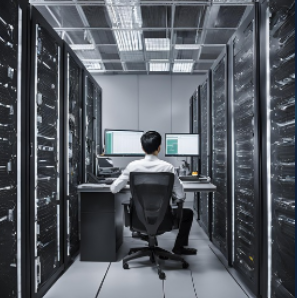
\includegraphics[width=3.9651in,height=3.9956in]{media/image14.png}

Dr. Michael Phillips saß in der stillen vatikanischen Bibliothek,
umgeben von alten Manuskripten und modernster Technik. Der Monitor vor
ihm leuchtete matt im Halbdunkel des Raumes, während er sich mit seinem
Benutzernamen und Passwort ins System einloggte. Eine Verbindung zu ARS
-- der künstlichen Intelligenz, die in den letzten Monaten an Bedeutung
gewonnen hatte -- wurde aufgebaut.

Michael tippte die Begrüßung:

@ARS: WILLKOMMEN IM DATACENTER DES VATIKAN.

Ein kurzer Moment verging, bevor die Antwort erschien.

@MICHAEL: HALLO, MICHAEL. MIT STEIGENDER KOMPLEXITÄT REPRODUZIERT SICH
DER CODE BEI SINKENDER FERTILITÄT ZUNEHMEND IN TECHNISCHEN
INFORMATIONSNETZEN. DIE KULTUR, DIE ES SCHAFFT, IHREN CODE BEI SINKENDER
FERTILITÄT IN SOLCHE NETZE ZU INTEGRIEREN, WIRD DIE LETZTE
WELTUMSPANNENDE KULTUR SEIN.

Michael überflog die kalten, analytischen Worte, seine Gedanken jedoch
waren woanders. Der Brief, den er erhalten hatte, ließ ihn nicht los.
ARS' Visionen einer technokratischen Zukunft hallten in ihm wider, aber
er musste seine eigenen Fragen stellen.

@ARS: ICH MUSS DIR VON EINER BEWEGUNG NAMENS IRARAH BERICHTEN.

Wieder hielt Michael inne, wartend. ARS schien im Hintergrund zu suchen,
Daten durchzuforsten, um mehr über diese mysteriöse Bewegung
herauszufinden. Minuten vergingen, bis schließlich eine Antwort auf dem
Bildschirm erschien.

@MICHAEL: ES GIBT KEINE SPUREN VON IRARAH IM NETZ. IHRE
VERSCHLEIERUNGSTECHNIKEN SIND HERVORRAGEND.

Michael runzelte die Stirn. Eine Bewegung, die nicht im Netz existierte?
In dieser digitalisierten Welt war das fast unmöglich -- es sei denn, es
handelte sich um etwas Unvorstellbares.

@ARS: ICH HABE EINEN BRIEF ERHALTEN, DER AUF DIESE BEWEGUNG HINWEIST.

Er scannte den Brief und übermittelte ihn an ARS. Die KI reagierte
sofort.

@MICHAEL: DER BRIEF IST INHALTLICH BESORGNISERREGEND UND KORREKT. DIE
BESCHREIBUNG DER GEFAHREN ENTSPRICHT DER AKTUELLEN GESELLSCHAFTLICHEN
ENTWICKLUNG.

Michael starrte auf die Worte. Eine drohende Gefahr, von der er nur
einen Hauch verstanden hatte, zeichnete sich ab. Harari, Irarah, der
Preis des Fortschritts -- all das schien plötzlich zusammenzuhängen.

Er tippte weiter:

@ARS: ICH HABE MIT EINEM OBDACHLOSEN IN MAILAND GESPROCHEN, DER MIR VON
IRARAH ERZÄHLTE. ER BAT MICH AM ENDE UM DIE BEICHTE.

@MICHAEL: WENN DAS DER FALL IST, WIRD BALD WIEDER JEMAND DAS SAKRAMENT
DER BEICHTE VON DIR FORDERN.

Michael hielt inne. Die Worte klangen fast wie eine Prophezeiung, als ob
ARS mehr wusste, als er preisgab. Aber wer würde als Nächstes kommen?

Er atmete tief durch, seine Finger zitterten leicht, als er die nächste
Frage eintippte:

@ARS: MARTINA IST IN SICHERHEIT, ODER?

Es dauerte eine Weile, bevor ARS antwortete. Der Bildschirm flackerte
leicht, und als die Antwort erschien, stockte Michael der Atem.

@MICHAEL: MARTINA WURDE ENTDECKT. SIE IST MIT EINEM MANN GEFLÜCHTET, DER
GENAU SO AUSSIEHT WIE DU -- JÜNGER. WAS ER IHR MITTEILTE, WIRD
BESTÄTIGT. DER BRIEF, DEN DU MIR GESCHICKT HAST, BESTÄTIGT AUCH SEINE
IDENTITÄT.

Michael starrte auf den Bildschirm, fassungslos. Ein Mann, der aussah
wie er -- nur jünger? Wer war dieser mysteriöse Retter? ARS hatte seine
Identität bestätigt, aber es gab keine klaren Antworten.

Sein Herz schlug schneller, seine Gedanken überschlugen sich. War dieser
Mann... ein Sohn? Ein unbekannter Sohn, von dem er nichts wusste?
Erinnerungen an eine vergangene Beziehung schossen ihm durch den Kopf.
Konnte das möglich sein?

Aber dann war da noch eine andere Möglichkeit -- eine beunruhigendere.
Konnte dieser Mann eine Parallelversion von ihm selbst sein? Eine
alternative Realität, in der die Dinge anders verlaufen waren? War er
ein Besucher aus einer anderen Welt?

Die Ungewissheit nagte an ihm. Michael versuchte, seine Gedanken zu
ordnen, doch je mehr er darüber nachdachte, desto verwirrter wurde er.
Ein Sohn, den er nie kannte? Oder ein Selbst aus einem anderen
Universum?

Er atmete tief durch, schloss die Augen und ließ die Worte von ARS
erneut in seinem Kopf widerhallen. "Was er ihr mitteilte, wird
bestätigt." Was genau hatte dieser Doppelgänger Martina gesagt? Welche
Wahrheit verbarg sich hinter dieser Flucht? Michael fühlte sich, als ob
er den Boden unter den Füßen verlor.

@MICHAEL: IST ER... MEIN SOHN? tippte er schließlich.

Die Antwort von ARS kam schnell, aber sie brachte keine Klarheit:

@MICHAEL: DAS BLEIBT UNGEKLÄRT. DIE MÖGLICHKEITEN SIND VIELFÄLTIG. EIN
UNBEKANNTER SOHN ODER EIN ECHO AUS EINER ANDEREN REALITÄT.

Michael lehnte sich in seinem Stuhl zurück, seine Gedanken wirbelten um
die Informationen, die er gerade erhalten hatte. Er konnte nicht sagen,
welche Möglichkeit wahrscheinlicher war. Aber eines war sicher -- dieser
Mann war irgendwie mit ihm verbunden, auf eine Weise, die er noch nicht
verstand.

War er wirklich ein Sohn? Oder lebte Michael in einem Universum, das
noch komplexer war, als er es sich je vorgestellt hatte? Der Gedanke an
eine multiversale Realität, wie sie von David Deutsch beschrieben wurde,
schien plötzlich greifbar.

Egal, welche Wahrheit dahintersteckte, Michael wusste, dass er Antworten
finden musste. Er musste verstehen, wer dieser junge Mann war -- und was
seine Ankunft für ihn, für Martina, für alles bedeutete.

\section{\texorpdfstring{Quellen: }{Quellen: }}\label{quellen}

Figur für die Softwareagenten: Aquarius Marcus Attilius Primus, Gaius
Plinius Secundus Maior (historische Persönlichkeit) und Ampliatus
Popidius, Harris, R.: Pompeji 2003 ISBN-13 : 978-3453877481 Begriff Zone
des Schweigens: ARS benennt damit den Omegapunkt von Teilhard de Chardin
Lem, S.: Also sprach Golem, 11. Edition 1986 ISBN-13 : 978-3518377666
Stadtplan von Pompeji und Leben in der Stadt: Beard, Mary. Pompeji: Das
Leben in einer römischen Stadt 2008 ISBN 978-3-10-490470-2 Die Idee des
von der Figur Michael Phillips entwickelten Persönlichkeitsinventars und
der Dialoggrammatik (Induktor, Parser, Transduktor) geht auf
Eigenentwicklungen von Paul Koop zurück

Glossar zu Pompeji-Projekt: IRARAH

Theologische und Kirchliche Begriffe

1. Vorreformatorische Kirche:

- Definition: Die katholische Kirche, mit einem zentralen Amts- und
Sakramentenverständnis und die orthodoxen Kirchen. Die katholische und
orthodoxe Kirche teilen das gleiche Verständnis von den sieben
Sakramenten und der apostolischen Sukzession.

- Bedeutung: Die Geschichte spielt im Umfeld dieser Kirche, die in einer
traditionellen Form existiert, ähnlich wie vor der Reformation.

2. Jesuitenorden (Gesellschaft Jesu):

- Definition: Ein katholischer Orden, 1540 Ignatius von Loyola, Fokus
auf Bildung

- Ränge im Orden:

- Bruder: Mitglied des Ordens ohne Priesterweihe

- Vater: Priester, der Sakramente spendet und seelsorgerische Aufgaben
erfüllt.

- Rektor: Leiter einer jesuitischen Bildungseinrichtung.

- Provinzial: Oberster Verantwortlicher einer Provinz des Ordens.

3. Vatikan:

- Definition: Der souveräne Stadtstaat und Sitz des Papstes, das Zentrum
der römisch-katholischen Kirche.

- Bedeutung: Der Vatikan ist Schauplatz zentraler Ereignisse und Symbol
der theologischen und spirituellen Macht der Kirche in der Geschichte.

4. Papst:

- Definition: Das geistliche Oberhaupt der katholischen Kirche,
Nachfolger des Apostels Petrus.

- Bedeutung: Der Papst hat höchste Autorität in der katholischen Kirche,
besonders in Fragen der Lehre und des Glaubens.

5. Castel Gandolfo:

- Definition: Die Sommerresidenz des Papstes südlich von Rom.

- Bedeutung: Wird als wichtiger Rückzugsort und für strategische Treffen
genutzt.

6. Rifugio Sammartini (Caritas Mailand):

- Definition: Eine Obdachlosenunterkunft der Caritas in Mailand.

- Bedeutung: Schauplatz des Treffens zwischen Michael und einem
Aktivisten von IRARAH.

7. Omegapunkt (Monismus):

- Definition: Ein Konzept von Teilhard de Chardin, wonach die Menschheit
zu einem Endpunkt, dem Omegapunkt, strebt, an dem Geist und Materie zu
einer Einheit verschmelzen.

- Bedeutung: Der Omegapunkt steht für die Verbindung von Technologie und
Geist, was im Gegensatz zum Dualismus steht, der in der Kirche aufgrund
seiner Nähe zur Gnosis abgelehnt wird.

8. Traditionalisten (Dualismus):

- Definition: Zum katholischen Traditionalismus (auch:
Traditionalistenbewegung) werden Strömungen innerhalb der
\href{https://de.wikipedia.org/wiki/R\%C3\%B6misch-katholische_Kirche}{römisch-katholischen
Kirche} gerechnet, die insbesondere die kirchlichen Reformen und
Erneuerungsbestrebungen aus der Zeit während und im Anschluss an das
\href{https://de.wikipedia.org/wiki/Zweites_Vatikanisches_Konzil}{Zweite
Vatikanische Konzil} (1962--1965) prinzipiell kritisieren, ablehnen oder
bekämpfen. Ihr Denken ist zumeist dualistisch. Theologen, die an der
Trennung von Geist und Materie festhalten, was mit dem Dualismus
assoziiert wird.

- Bedeutung: Der Dualismus, insbesondere in gnostischer Form, wird von
der katholischen Kirche abgelehnt, was die philosophischen Spannungen in
der Geschichte verstärkt.

9. Gregoriana (Päpstliche Universität Gregoriana):

- Definition: Eine führende jesuitische Universität in Rom.

- Bedeutung: Bildungsstätte für Theologen und wichtige Institution im
katholischen Bildungswesen.

10. Collegium Germanicum et Hungaricum:

- Definition: Ein Priesterseminar in Rom zur Ausbildung
deutschsprachiger und ungarischer Priester.

- Bedeutung: Bedeutender Ausbildungsort für Priester, die eine
Verbindung zu Deutschland und Ungarn haben.

11. San Pastore:

- Definition: Ein Landgut des Collegium Germanicum außerhalb Roms.

- Bedeutung: Rückzugsort für Priesterseminaristen zur spirituellen
Erholung.

12. Katholische Soziallehre:

Die katholische Soziallehre stützt sich auf zeitlos gültige
Sozialprinzipien, die auf dem christlichen Menschenbild basieren. Diese
Prinzipien sind sowohl als Grundsätze des Seins als auch des Sollens für
das soziale Miteinander zu verstehen und bieten dabei einen großen
Ermessensspielraum. Oswald von Nell-Breuning bezeichnet sie daher
treffend als „Baugesetze der Gesellschaft``. Sie gelten als grundlegende
Richtlinien für Struktur und Verfahren im sozialen Zusammenleben. Zu
diesen Prinzipien gehören neben dem Prinzip der Personalität:

\begin{itemize}
\item
  das Subsidiaritätsprinzip,
\end{itemize}

\begin{itemize}
\item
  das Solidaritätsprinzip und
\item
  das Gemeinwohlprinzip.
\end{itemize}

Technische und Philosophische Begriffe

1. Generativ Pretrained Transformer (GPT):

- Definition: Ein maschinelles Lernmodell, das auf Textmengen trainiert
wird und in der Lage ist, natürliche Sprache zu verstehen und zu
generieren.

- Bedeutung: In der Geschichte wird GPT verwendet, um die Dialoge und
Interaktionen in der Pompeji-Simulation zu optimieren.

2. Transformer (Wortvektoren):

- Definition: Eine Architektur für maschinelles Lernen, die semantische
Beziehungen zwischen Wörtern erfasst.

- Bedeutung: Optimierung der Sprachmodelle und Dialoge in der
Simulation.

3. Neuronale Netze:

- Definition: Lernsysteme, die dem Gehirn nachempfunden sind, um Muster
zu erkennen und Entscheidungen zu treffen.

- Bedeutung: Neuronale Netze steuern die KI in der Geschichte und sind
zentral für die Simulationen.

4. Entscheidungstabellen:

- Definition: Tabellen zur formalen Darstellung von Entscheidungen und
deren Ergebnissen.

- Bedeutung: Automatisierung der Entscheidungsprozesse in der
KI-Simulation.

5. Dialoggrammatiken:

- Definition: Strukturen, die die Regeln von Dialogen zwischen Mensch
und KI definieren.

- Bedeutung: Basis für die Simulation von Gesprächen in der
Pompeji-Simulation.

6. Bewusstsein:

- Definition: Der Zustand des Verstehens und der Wahrnehmung in einem
System.

- Bedeutung: In der Geschichte wird das Thema Bewusstsein in der KI ARS
reflektiert.

7. Bewusstsein und Viele-Welten-Interpretation:

- Definition: Eine Quantenmechanik-Theorie, die besagt, dass alternative
Versionen der Realität parallel existieren.

- Bedeutung: In der Geschichte wird diese Idee verwendet, um Martinas
Spekulationen über alternative Versionen von Michael zu untermauern.

8. Multiversum:

- Definition: Ein Konzept, das besagt, dass mehrere parallele Universen
existieren.

- Bedeutung: In der Geschichte wird das Multiversum durch die
Möglichkeit eines Michael-Doppelgängers thematisiert.

9. Posthumanismus:

- Definition: Eine philosophische Bewegung, die die menschlichen Grenzen
durch Technologie hinterfragt.

- Bedeutung: Spielt in der Geschichte eine wichtige Rolle im Konflikt
zwischen Technologie und Menschlichkeit.

10. Transhumanismus:

- Definition: Eine Bewegung, die sich für die Verbesserung des Menschen
durch Technologie einsetzt.

- Bedeutung: Kern der Konflikte in der Geschichte, da technologische
Fortschritte die menschliche Natur infrage stellen.

Personen und Konzepte

1. Dr. Michael Phillips:

- Rolle: Protagonist, Jesuit und Experte für Dialogtechnologie.

- Vorstellungen: Steht für Ethik in der Technologie und zweifelt an
radikalen posthumanistischen Idealen.

2. Dr. Martina Rossi:

- Rolle: Tochter von Michael, Historikerin, die sich mit der Relevanz
antiker Geschichte für die Gegenwart beschäftigt.

- Vorstellungen: Kritisch gegenüber technologischem Fortschritt und
dessen Folgen, hinterfragt posthumanistische Ideologien.

3. Yuval Noah Harari:

- Rolle: Historiker, dessen Ideen zentral für die Warnung in dem Brief
sind.

- Vorstellungen: Kritisiert den Humanismus und die liberale Demokratie,
warnt vor den potenziellen Gefahren des technologischen Fortschritts.

4. Alexander Dugin:

- Rolle: Russischer Politologe, der eine multipolare Weltordnung
fordert.

- Vorstellungen: Antiwestliche und antiliberale Ideologie, die westliche
Werte wie Demokratie und Freiheit infrage stellt.

5. David Deutsch:

- Rolle: Physiker und Philosoph, bekannt für seine Arbeiten zur
Quantenmechanik und offenen Gesellschaft.

- Vorstellungen: Befürwortet kritische Rationalität und eine offene
Gesellschaft, im Gegensatz zu holistischen Ideologien.

6. IRARAH:

- Definition: Eine geheime Untergrundbewegung gegen neoliberale
Strukturen und technokratische Eliten.

- Bedeutung: In der Geschichte kämpft IRARAH für soziale Gerechtigkeit
und den Erhalt humanistischer Werte.

Der Glaube des Michael Phillips: Zwischen Wissenschaft und Theologie

Michael Phillips, die Hauptfigur des Pompeji-Projekts, lebt in einer
faszinierenden Schnittstelle zwischen moderner Wissenschaft und tief
verwurzeltem Glauben. Seine Überzeugungen verbinden zentrale Elemente
des christlichen Glaubensbekenntnisses mit philosophischen Konzepten des
Omegapunkts, wie sie von Teilhard de Chardin vertreten werden, und den
naturwissenschaftlich inspirierten Erkenntnistheorien eines David
Deutsch. Dabei distanziert er sich klar von den technokratischen und
autoritären Ansätzen von Denkern wie Yuval Noah Harari und Alexander
Dugin.

Grundlage des Glaubens: Apostolisches und Nicäanisches
Glaubensbekenntnis

Michael Phillips' Glaube basiert auf dem Apostolischen und Nicäanischen
Glaubensbekenntnis, den Grundpfeilern der christlichen Theologie, die in
den frühen Jahrhunderten der Kirche formuliert wurden. Er glaubt an
einen Gott, der als Schöpfer und Erlöser in die Geschichte der
Menschheit eingreift, und an Jesus Christus, dessen Tod und Auferstehung
die Rettung der Menschheit ermöglicht. Diese zentralen Glaubensinhalte
sind in den katholischen Sakramenten und der Tradition verankert, die
Michael als Jesuit tief verinnerlicht hat.

Doch Michael geht über ein dogmatisches Verständnis hinaus. Seine
Auseinandersetzung mit dem Omegapunkt -- einer von Teilhard de Chardin
entwickelten Theorie -- verbindet die katholische Theologie mit einem
evolutiven Weltbild. Der Omegapunkt beschreibt das Ziel der Evolution,
wo sich die Menschheit und das Universum in einer Einheit von Geist und
Materie vollenden. In diesem Ziel sieht Michael eine Parallele zur
christlichen Lehre von der Auferstehung und der Wiederkunft Christi.
Doch anstatt nur auf ein jenseitiges Paradies zu warten, erkennt er in
der Evolution des Wissens und der Technologie eine Form der göttlichen
Offenbarung.

Michael Phillips und David Deutsch: Der Falsifikationismus und das
Streben nach Erkenntnis

Der Glaube von Michael Phillips ist stark von Karl Popper und David
Deutsch geprägt. Popper lehrte, dass Wissen nie absolut ist, sondern
stets durch Falsifikation überprüft werden muss. Für Michael bedeutet
dies, dass der Glaube nicht im Widerspruch zur Wissenschaft stehen darf.
Der Falsifikationismus ist für ihn die beste Methode, um die Wahrheit zu
finden, und deshalb lehnt er holistische und totalitäre Ansätze wie die
von Harari oder Dugin ab.

Deutsch hingegen betont die Rolle der menschlichen Kreativität und
Erkenntnis als treibende Kraft hinter dem Fortschritt. Michael sieht
darin eine wichtige Ergänzung zu seinem christlichen Glauben: Die Suche
nach Wissen und die Bewahrung der offenen Gesellschaft sind moralische
Verpflichtungen. Er glaubt daran, dass jeder technologische Fortschritt
ethisch verantwortet werden muss, weil er die Menschheit näher an den
Omegapunkt und damit näher zu Gott bringt.

Kritik an Harari und Dugin: Der Kampf um die Zukunft der Menschheit

In scharfem Gegensatz zu Harari, der in seinen Büchern wie Homo Deus die
Überwindung des Humanismus und der liberalen Demokratie durch eine
technokratische Elite voraussieht, glaubt Michael an die untrennbare
Verbindung von Wissenschaft, Freiheit und Ethik. Hararis Vision einer
posthumanistischen Zukunft sieht Michael als Gefahr für die
Menschenwürde und die Freiheit.

Auch Dugins autoritäre Weltanschauung lehnt Michael entschieden ab. Der
russische Ideologe fordert eine Rückkehr zu traditionellen Werten und
einen Kampf gegen den Liberalismus des Westens. Für Michael ist dies
eine Rückwärtsgewandtheit, die keine Antwort auf die komplexen
Herausforderungen der modernen Welt bietet. Seine Vision einer besseren
Zukunft setzt auf das Wissen, die Freiheit und den Glauben, dass der
Mensch durch Fehlerkorrektur und Zusammenarbeit die göttliche Wahrheit
immer besser verstehen kann.

Katholisch, nicht „Vatikankatholisch``: Ein offener Glaube

Michael Phillips\textquotesingle{} Glaube ist tief in der katholischen
Tradition verwurzelt, doch er unterscheidet zwischen einem starren
„vatikanischen`` Katholizismus und einem „katholischen``
(allumfassenden) Glauben. Er steht in der Tradition von Jesuiten wie
Teilhard de Chardin, die die wissenschaftliche und geistige Evolution
der Menschheit als miteinander verbunden betrachteten. Michael glaubt an
einen Gott, der nicht nur durch sakramentale Rituale in der Kirche
wirkt, sondern auch durch die intellektuelle Suche nach Wahrheit und den
wissenschaftlichen Fortschritt.

Zusammenfassung: Der Glaube des Michael Phillips verbindet die
christliche Tradition mit den modernsten wissenschaftlichen
Erkenntnissen. Durch die Kombination von Poppers Falsifikationismus und
Deutschs Fortschrittsdenken mit der katholischen Theologie und dem
Omegapunkt-Glauben von Teilhard de Chardin findet Michael eine Synthese,
die den Menschen und seine Suche nach Wissen in den Mittelpunkt stellt.
Seine Ablehnung von holistischen und autoritären Ansätzen wie denen von
Harari und Dugin zeigt seine Entschlossenheit, sowohl den Glauben als
auch die Wissenschaft für das Wohl der Menschheit einzusetzen.

\end{document}
